\chapter{پیاده‌سازی و ارزیابی روش پیشنهادی}
\newpage
‎\renewcommand{\baselinestretch}{2}\normalsize‎
\label{ExperimentResults}

در این فصل به ارزیابی روش پیشنهادی بر روی مسائل مختلف همچون   شناسایی سیستم و پیش‌بینی پرداخته شده است. مساله شناسایی سیستم یکی از مسائل معیار و معروف در حوزه الگوریتم‌های یادگیری توزیع‌شده مبتنی بر شبکه‌های تطبیقی است و در این رساله، برای مساله پیش‌بینی بر روی پیش‌بینی وضعیت بازار بورس سهام در روزهای آینده متمرکز شده‌ایم. در بازار بورس سهام روزانه حجم زیادی از اطلاعات و تراکنش‌ها تولید می‌شود که گاها به تحلیل‌های آنی و سریع نیاز دارد تا‌‌ با پیش‌بینی‌های دقیق امکان انجام معامله‌های هوشمندانه و پرسود میسر شود. در بخش‌های بعدی نشان داده شده است رویکرد یادگیری توزیع‌شده پیشنهادی قادر است پیش‌بینی را به درستی با دقت بالا و نرخ خطا پایین بر روی داده‌های بازار بورس سهام ایران انجام دهد.

به دلیل محدودیت‌ در دسترسی به زیرساخت‌های فیزیکی پیچیده و همچنین سهولت در ارزیابی همه‌جانبه رویکرد پیشنهادی، پیاده‌سازی رویکرد پیشنهادی در یک محیط شبیه‌سازی‌شده انجام شده است. در ادامه این فصل، شبیه‌ساز مورد استفاده معرفی خواهد شد. سپس روش‌هایی که روش پیشنهادی با آن‌ها مقایسه شده است، معرفی می‌گردند. همچنین به منظور ارزیابی روش پیشنهادی با سایر روش‌ها، چندین معیار معرفی خواهد شد. در انتها نتایج بدست آمده از رویکرد پیشنهادی با سایر روش‌‌ها به همراه تجزیه و تحلیل نتایج و بیان نقاط قوت و ضعف هر روش ارائه می‌گردد. 

\section{شبیه‌سازی شبکه‌های تطبیقی توزیع‌شده با \lr{SimGrid}}\label{SimGrid}

در این رساله، برای ارزیابی و مقایسه نتایج، از چارچوب شبیه‌سازی \lr{SimGrid} \cite{SimGrid2014} استفاده می‌کنیم که توانایی بالایی در منعکس کردن رفتار واقعی سیستم یا پروتکل‌های توزیع‌شده پیشنهادی دارد. شبیه‌ساز \lr{SimGrid} یک چارچوب نرم‌افزاری قدرتمند و انعطاف‌پذیر است که برای شبیه‌سازی، مدل‌سازی و آنالیز سیستم‌های توزیع‌شده طراحی شده است. این سیستم‌ها شامل مجموعه‌ای از رایانه‌ها و منابع شبکه‌ای هستند که به صورت همگام در انجام یک مجموعه وظایف محاسباتی مشارکت می‌کنند. \lr{SimGrid} به طور خاص برای پژوهشگران و توسعه‌دهندگان ایجاد شده است تا بتوانند به راحتی رفتار و عملکرد برنامه‌های توزیع‌شده را در محیط‌های مختلف و با تنظیمات گوناگون مورد بررسی و ارزیابی قرار دهند.

یکی از نقاط قوت \lr{SimGrid} این است که می‌تواند بدون نیاز به اجرای واقعی برنامه‌ها بر روی یک زیرساخت فیزیکی پیچیده، رفتار و کارایی آن‌ها را در یک محیط شبیه‌سازی شده مطالعه کند. این قابلیت به پژوهشگران اجازه می‌دهد تا سناریوهای مختلفی از جمله بارهای کاری متفاوت، توپولوژی‌های شبکه متنوع، و تغییرات در سطح منابع را شبیه‌سازی کنند. این شبیه‌ساز با استفاده از یک موتور شبیه‌سازی کارآمد، به کاربران امکان می‌دهد تا با دقت بالا نتایج قابل اعتمادی از شبیه‌سازی‌های خود به دست آورند. این چارچوب به دلیل انعطاف‌پذیری بالا و قابلیت‌های گسترده‌ای که ارائه می‌دهد، به یکی از ابزارهای استاندارد در زمینه شبیه‌سازی سیستم‌های توزیع‌شده تبدیل شده است و برای طیف گسترده‌ای از حوزه‌های محاسباتی توزیع‌شده همانند، محاسبات گرید، محاسبات \lr{P2P}، محاسبات ابری، محاسبات مه، محاسبات سنگین با \lr{MPI} و \lr{MapReduce} مورد استفاده قرار می‌گیرد. مدل‌های شبیه‌سازی \lr{SimGrid} دقیق می‌باشند و به صورت تئوری و تجربی ارزیابی و اعتبارسنجی شده‌ و مقیاس‌پذیر می‌باشند. پیاده‌سازی آنها سریع بوده و به حافظه کمی نیاز دارد. در نتیجه به راحتی امکان اجرای سریع شبیه‌سازی‌های \lr{SimGrid} بر روی یک دستگاه فراهم است.

\subsection{مولفه شبیه‌سازی \lr{SMPI}}\label{SMPI_Sec}

یکی از مؤلفه‌های اصلی و بسیار کاربردی \lr{SimGrid}،
 مولفه \lr{SMPI} (\lr{Simulate MPI}) است که به طور خاص برای شبیه‌سازی برنامه‌های \lr{MPI} طراحی شده است. همانطور که قبلا اشاره شده است، \lr{MPI} یک استاندارد معروف برای برنامه‌نویسی موازی است که به فرآیندها اجازه می‌دهد تا از طریق ارسال و دریافت پیام با یکدیگر ارتباط برقرار کنند. این استاندارد به طور گسترده در محاسبات با کارایی بالا \footnote{\lr{HPC}} استفاده می‌شود. مولفه \lr{SMPI} به کاربران امکان می‌دهد تا برنامه‌های \lr{MPI} را بدون نیاز به یک کلاستر فیزیکی یا محیط محاسباتی گسترده اجرا و شبیه‌سازی کنند. این ابزار قابلیت اجرای برنامه‌های \lr{MPI} را در مقیاس بزرگ فراهم می‌کند و به کاربران اجازه می‌دهد تا با تغییر پارامترهای مختلف شبیه‌سازی، تأثیرات آن‌ها را بر عملکرد برنامه‌ها بررسی کنند. با استفاده از این ابزارها، دانشجویان و پژوهشگران می‌توانند به سرعت و بدون نیاز به زیرساخت‌های پیچیده، برنامه‌های موازی خود را توسعه داده و آن‌ها را در سناریوهای مختلف تست و بهینه‌سازی کنند و به راحتی مقیاس‌پذیری و عملکرد برنامه‌های خود را در محیط‌های شبیه‌سازی بررسی و بهترین راهکارها را برای بهبود کارایی آن‌ها پیدا کنند.
 \subsection{مراحل انجام شبیه‌سازی}
شکل \ref{SMPI}،  نمای کلی از نحوه کارکرد \lr{SimGrid} و \lr{SMPI} را در فرآیند شبیه‌سازی یک برنامه \lr{MPI} به تصویر می‌کشد. این شکل مراحل مختلف شبیه‌سازی را از دیدگاه یک برنامه کاربردی تا اجرا در محیط شبیه‌سازی نشان می‌دهد. در ادامه، روند انجام یک شبیه‌سازی ساده با \lr{SMPI} توضیح داده شده است.

\begin{figure}
	\centering
	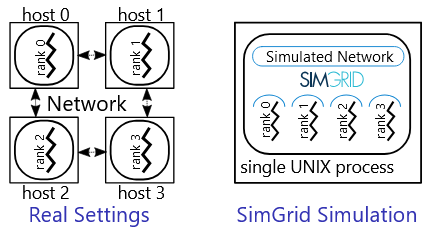
\includegraphics[scale=1.6]{SMPI.PNG}
	\caption{نمای کلی از نحوه کارکرد \lr{SimGrid} و \lr{SMPI} را در فرآیند شبیه‌سازی یک برنامه \lr{MPI}}\label{SMPI}
\end{figure}


\begin{itemize}
	\item نوشتن کد برنامه \lr{MPI}
	
	ابتدا باید یک برنامه ساده \lr{MPI} نوشته شود. این برنامه می‌تواند به زبان \lr{C} یا \lr{C++} نوشته شود و از توابع استاندارد \lr{MPI} برای ارتباط بین فرآیندها استفاده کند. به عنوان مثال، یک برنامه ساده که پیام‌های بین دو فرآیند را ارسال و دریافت می‌کند.
	
	\item کامپایل برنامه با  \lr{SMPI}
	
	پس از نوشتن برنامه، از کامپایلر \lr{smpicc} برای کامپایل کردن کد استفاده می‌شود. این کامپایلر همانند \lr{mpicc} عمل می‌کند اما برنامه را برای اجرای شبیه‌سازی در محیط \lr{SimGrid} آماده می‌کند.
	
\begin{figure*}
	\centering
	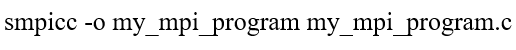
\includegraphics[scale=1]{Form3.PNG}
\end{figure*}
	
	\item ایجاد فایل پیکربندی 
	
	در صورت نیاز، می‌توان یک فایل پیکربندی برای تعیین پارامترهای شبیه‌سازی مانند تعداد فرآیندها، تعریف توپولوژی شبکه، مدل‌های مصرف انرژی، مدل‌های پردازشی، پیکربندی‌های شبیه‌سازی خاص و پارامترهای مرتبط با زمان‌بندی، ایجاد کرد.  برای تعریف توپولوژی شبکه می‌توان با استفاده از یک فایل \lr{XML}، لینک‌های ارتباطی و پهنای باند گره‌ها را مشخص کرد.

 همچنین با استفاده از \lr{SMPI} می‌توان مصرف انرژی فرآیندها را شبیه‌سازی کرد. این بخش از فایل پیکربندی می‌تواند شامل پارامترهایی برای تعیین میزان مصرف انرژی در هر گره و ارتباطات بین گره‌ها باشد. مدل‌های پردازشی مختلفی را برای شبیه‌سازی عملکرد پردازنده‌ها تعریف کرد. این مدل‌ها می‌توانند شامل زمان‌بندی فرآیندها، مدل‌های حافظه و غیره باشند. پیکربندی‌های خاص شامل تنظیمات خاصی مانند فعال یا غیرفعال کردن گزارش‌های خاص، تغییر سطح دقت شبیه‌سازی و یا تنظیم پارامترهای دقیق‌تری برای مدل‌های شبیه‌سازی است. پارامتر \lr{tracing:yes} به معنای فعال کردن قابلیت ردیابی و \lr{surf/precision:1e-9} به معنای تنظیم دقت شبیه‌سازی است. پارامترهای مرتبط با نوع زمان‌بندی فرآیندها و تخصیص منابع را مشخص کرد. این پارامترها تعیین می‌کنند که چگونه فرآیندها به منابع سیستم دسترسی دارند و چگونه منابع بین آن‌ها تقسیم می‌شود.
	\begin{figure*}
		\centering
		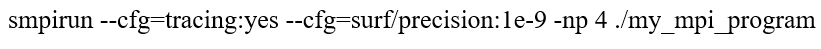
\includegraphics[scale=0.9]{Form1.PNG}
	\end{figure*}
	
	\item اجرای شبیه‌سازی با \lr{SMPI}
	
	برای اجرای برنامه، از دستور \lr{smpirun} استفاده می‌شود. این دستور تعداد فرآیندها و سایر پارامترهای شبیه‌سازی را مشخص می‌کند. پارامتر \lr{-np 2} تعداد فرآیندهایی که باید اجرا شوند را تعیین می‌کند.
	
	\item مشاهده و تحلیل نتایج
	
	پس از اجرای شبیه‌سازی، خروجی برنامه در ترمینال نمایش داده می‌شود. این خروجی می‌تواند شامل نتایج محاسبات، پیام‌های ارسال و دریافت شده، و زمان‌های اجرای فرآیندها باشد. این نتایج می‌توانند برای تحلیل عملکرد برنامه استفاده شوند.
	
\end{itemize}
\subsection{ابزار \lr{FBSPonMPI}}
در این رساله با کمک نرم‌افزار شبیه‌سازی \lr{SimGrid} ابزاری به نام \lr{FBSPonMPI} به‌منظور شبیه‌سازی پردازش مورد نظر طراحی شده است (شکل \ref{Tool} را ببینید). جزئیات بخش‌های آن‌ در ادامه به صورت مختصر شرح داده می‌شوند. 
\begin{figure*}[!h]
	\centering
	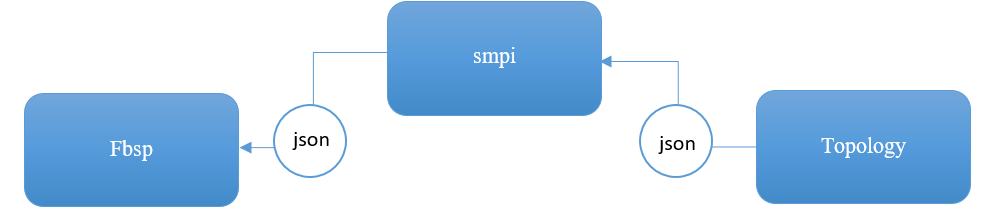
\includegraphics[width=16cm]{MyTool.png}
	\caption{شمای کلی ابزار \lr{FBSPonMPI}}
	\label{Tool}
\end{figure*}
\subsubsection{توپولوژی}
بخش اول ابزار از یک کد پایتون  با مجموعه کلاس‌های \lr{Data}، \lr{ICSCluster}، \lr{SimgridXML} و \lr{Topology}  تشکیل شده است. کلاس \lr{Topology} وظیفه ساخت توپولوژی شبکه بر اساس پارامترهای ورودی را دارد. ساخت این توپولوژی می‌تواند به‌صورت تصادفی یا بر اساس تنظیمات مورد نظر باشد. ماتریس مجاورت توپولوژی ایجادشده در این بخش در اختیار بخش‌های دیگر ابزار قرار می‌گیرد. کلاس \lr{SimgridXML} وظیفه ایجاد فایل پیکربندی \lr{simgrid} بر اساس توپولوژی ایجاد شده را بر عهده دارد.  این پیکربندی نحوه و نوع اتصال فرآیندها به یکدیگر در شبکه را مشخص می‌کند. این پیکربندی برای شبیه‌سازی عملکرد و رفتار برنامه‌های محاسبات توزیع‌شده با استفاده از \lr{SimGrid} مورداستفاده قرار می‌گیرد. 

در کلاس \lr{ICSCluster} منطقه‌بندی شبکه ایجاده شده در مرحله قبل با استفاده از روش خوشه‌بندی ساختار-محتوایی انجام خواهد شد. در این مورد، ساختار به معنای اتصالات و روابط گره‌ها و محتوا به معنای ویژگی‌های مرتبط با گره‌ها است. خروجی این کلاس یک فایل \lr{json} می‌باشد که شامل تعداد منطقه‌ها و اعضای آن است. این فایل نیز توسط بخش دوم ابزار مورداستفاده قرار می‌گیرد. کلاس \lr{Data} وظیفه تولید یا آماده‌سازی داده‌های اولیه برای پردازنده‌ها را بر عهده دارد و خروجی آن به صورت ‌یک فایل \lr{json} است که در اختیار هر پردازنده قرار خواهد گرفت. 

\subsubsection{\lr{SMPI}}
این بخش، هسته اصلی ابزار \lr{FBSPonMPI} است که توسط مولفه \lr{SMPI} از شبیه‌ساز \lr{SimGrid} توسعه‌ یافته است. این مولفه امکان شبیه‌سازی عملکرد برنامه‌های \lr{MPI} را فراهم می‌کند و به کاربران امکان می‌دهد بدون نیاز به سخت‌افزار واقعی، عملکرد برنامه‌های خود را در یک محیط شبیه‌سازی‌شده آزمایش کنند. شکل \ref{SMPI_ph} پردازش انجام‌شده در این بخش را نشان می دهد که از سه قسمت اصلی \lr{adapt}، \lr{communication}  و \lr{combine} تشکیل شده است.   داده، توپولوژی شبکه، اطلاعات مربوط به منطقه‌ها و فایل پیکربندی که در بخش قبل ایجاد شده‌اند در اختیار \lr{smpi} قرار می‌گیرند و پردازش توزیع‌شده به‌صورت شبیه‌سازی‌شده اجرا می‌شود و نتایج بدست آمده توسط هر پردازنده در یک فایل \lr{json} قرار می‌گیرند تا در انتهای فرآیند یادگیری توزیع‌شده تجمیع شده و برای رسم نمودارها مورد استفاده قرار گیرند.

\begin{figure*}[!h]
	\centering
	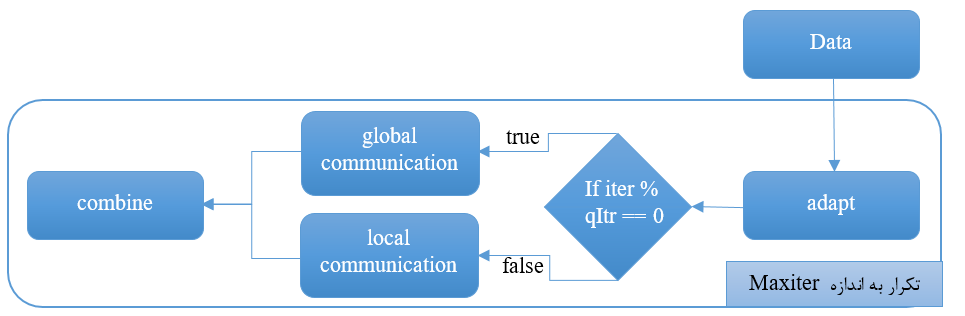
\includegraphics[width=16cm]{SMPI_Phases.png}
	\caption{مراحل پردازش در بخش \lr{SMPI}}
	\label{SMPI_ph}
\end{figure*}

در بخش \lr{FBSP} ابزار، تمامی داده‌های تولیدشده توسط \lr{smpi} برای تحلیل و رسم نمودار مورد استفاده قرار می‌گیرند.



\section{پیاده‌سازی محیط غیرایستا در آزمایشات}
یک الگوریتم یادگیری تطبیقی باید در هر محیطی توانایی یادگیری بالایی داشته باشد. در برخی از محیط‌ها مدل سیستم در طول زمان ثابت است و دست‌خوش تغییرات نمی‌شود. در این حالت با یک محیط ایستا\footnote{\lr{Stationary}} روبه‌رو هستیم. در حالتی که مدل سیستم ثابت نباشد و در طول زمان تغییر کند، یک محیط غیرایستا\footnote{\lr{non-Stationary}} خواهیم داشت. در اکثر موارد، کارایی و عملکرد یادگیری الگوریتم‌های تطبیقی انتشاری در محیط‌های غیرایستا با مشکل مواجه خواهد شد. به منظور بررسی توانایی ردیابی الگوریتم‌های یادگیری پیشنهادی، در آزمایشات از مدل ردیابی \ref{Track} استفاده شده است.
\begin{equation}
	Tracking\quad model:
	\begin{cases} 
		w_{o,t}=w_o+\omega_t\\
		\omega_t=0.9\omega_{t-1}+q_t
	\end{cases}
	\label{Track}
\end{equation}
که $q_t$ مجموعه‌ای از آشفتگی‌های \footnote{\lr{Perturbations}} مستقل با توزیع یکسان \footnote{\lr{Independent and Identically Distributed (iid)}} هستند که دارای میانگین صفر و ماتریس کوواریانس $Q$ می‌باشد و این مجموعه در هر تکرار مستقل از رگرسیون‌های ورودی و نویز خروجی است. پارامتر $Q$ به صورت $\sigma_q^2 I$ تعریف می‌شود و مقدار $\sigma_q^2$ برابر $10^{-4}$ است. در آزمایشات، عملکرد الگوریتم‌های یادگیری پیشنهادی در محیط غیرایستا در شرایطی کاملا یکسان و همانند محیط ایستا مورد بررسی قرار می‌گیرند. 
\section{نویزهای گاوسی و غیر گاوسی استفاده شده در آزمایشات}
وجود نویزهای مختلف در محیط پیاده‌سازی شبکه غیرقابل اجتناب است. نویزهای می‌توانند گاوسی یا غیرگاوسی باشند. ‌‌نویز گاوسی یک نویز استاتیکی است که از تابع توزیع چگالی احتمال نرمال یا همان تابع گاوسی پیروی می‌کند و مقادیر این نویز، توزیع گاوسی دارند. نویز غیرگاوسی از الگوی متقارن و زنگی شکل توزیع گاوسی منحرف می‌شود و از منابع نویز غیرتعادلی ناشی می‌شود. نویزهای غیرگاوسی حاکی از رخدادهای شدید در دامنه هستند که در نویز گاوسی وجود ندارند و رفتارشان به شدت تغییر می‌کند. در اغلب مطالعات به دلیل سادگی تشخیص و امکان دستیابی به برخی نتایج تحلیلی هنگام کار با نویزهای گاوسی، منبع نویز گاوسی در نظر گرفته می‌شود. عمدتاً به دلیل مشکلاتی که در کار با نویزهای غیرگاوسی وجود دارد، استفاده از آن‌ها به ندرت اتفاق می‌افتد. در این رساله، نویزهای غیر گاوسی با توزیع آلفا پایدار\footnote{\lr{$\alpha$-stable distribution}} و گاوسی آمیخته\footnote{\lr{Mixture Gaussian}} مدل‌سازی شده‌اند.

همان‌طور که ذکر شد، یکی از نویزهای غیرگاوسی که نویز پایدار $\alpha$ یا $\alpha-stable$ نامیده می‌شود از طریق توزیع $V_{\alpha-stable}(\alpha_{\nu},\beta_\nu,\gamma_{\nu},\delta_\nu)$ \cite{alphastable} مدل شده است و تابع مشخصه آن توسط رابطه \ref{alpha} تعریف می‌گردد:
\begin{equation}\label{alpha}
	\log \phi(t)=
	\begin{cases}
		-\gamma_{\nu}^{\alpha_{\nu}}|t|^\alpha_\nu\{1-i\beta_\nu sign(t)\tan\frac{\pi\alpha_\nu}{2}\}+i\delta_\nu t,\qquad\alpha_\nu\ne1\\
		-\gamma_\nu|t|\{1+i\beta_\nu sign(t)\frac{2}{\pi}\log|t|\}+i\delta_\nu t   \quad\qquad \alpha_\nu=1,
	\end{cases}
\end{equation}
که $\alpha_{\nu}$ پارامتر توانی است که در بازه $]0,2)$ قرار دارد. پارامتر مکانی $\delta_\nu\in \mathbb{R}$ توزیع را به سمت چپ یا راست شیفت می‌دهد. پارامتر مقیاس $\gamma_{\nu}>0$ توزیع را در حدود $\delta_\nu$ فشرده یا گسترش می‌دهد و پارامتر تقارن $\beta_\nu\in \left(-1,1\right]$ چولگی \footnote{\lr{Skewed}} توزیع را تعیین می‌کند. هنگامی که $\beta_\nu$ مثبت است، توزیع به سمت راست منحرف می شود و هنگامی که منفی است توزیع به سمت چپ منحرف می‌شود. زمانی‌که $\beta_\nu=0$، توزیع متقارن است \cite{alphastable_1999} و \cite{alphastable}.

همچنین، نویز گاوسی آمیخته به صورت زیر مدل شده است:
\begin{equation}
	(1-\theta)\mathcal{N}(\mu_1,\sigma_1^2)+\theta\mathcal{N}(\mu_2,\sigma_2^2)
\end{equation}
به منظور تولید نویز تکانشی\footnote{\lr{Impulsive noise}} یا داده‌های پرت بزرگ، باید پارامتر $\theta$ با یک مقدار کوچک تنظیم شود و $\sigma_1^2<<\sigma_2^2$ باشد. پارامتر مدل نویز برداری به صورت $V_{mix}(\mu_1,\mu_2,\sigma_1^2,\sigma_2^2,\theta)$ تعریف می‌شود. 
\section{توابع خطا بررسی‌شده در آزمایشات}
تابع خطا نقش بسزایی در کارایی و همگرایی الگوریتم‌های یادگیری انتشار دارد. در نتیجه انتخاب یک تابع خطای متناسب با مساله کاربردی و نوع نویزهای محیطی بسیار مهم و قابل توجه است. در طراحی تابع هزینه استفاده شده در فرایند یادگیری الگوریتم \lr{DSGD} معمولی از مربع خطا با فرم میانگین (امیدریاضی) $E\{l(e)\}=E\{e^2\}$ استفاده شده است. 

به منظور مقاوم‌سازی الگوریتم \lr{DSGD} در برابر انواع نویزهای محیطی در طراحی تابع هزینه آن انواع توابع خطا از جمله  \lr{pseudo-Huber loss}، \lr{Geman-McClure loss}، \lr{welsch loss} و \lr{cauchy loss} را مورد بررسی قرار داده‌ایم. تابع خطا  شبه‌هابر یا \lr{pseudo-Huber loss} تقریب نرمی از خطا هابر است که پیوسته و مشتق‌پذیر می‌باشد. تابع هزینه در الگوریتم پیشنهادی \lr{Robust Diffusion SGD} (\lr{RِDSGD}) بر اساس تابع خطا شبه‌هابر طراحی شده است که فرم میانگین آن به صورت زیر تعریف می‌شود:
\begin{equation}
	E\{l_\delta(e)\}=E\{\delta^2(\sqrt{1+(\frac{e}{\delta})^2}-1)\}
\end{equation}

که $\delta$ یک پارامتر اضافی برای کنترل شیب در زمان بروز خطاها با مقادیر بزرگ است. مزیت اصلی خطا شبه‌هابر این است که تابع آن دو بار مشتق‌پذیر بوده و نرم است؛ در حالی‌که خطا هابر غیرمحدب است و ممکن است الگوریتم‌های بهینه‌سازی در کمینه‌های محلی گیر کنند. 

شکل \ref{lossFun} منحنی رفتار برخی از توابع خطا از جمله تابع مربع خطا، خطا‌ شبه‌هابر، خطا \lr{welsch}، خطا \lr{Geman-McClure} و خطا \lr{cauchy} در مقابل مقادیر مختلف خطا نشان می‌دهد. در این شکل، پارامتر $\delta$ در خطا شبه‌هابر و پارامتر $c$ در خطا \lr{Geman-McClure} با مقدار $0.8$ تنظیم شده‌اند. همان‌طور که مشاهده می‌شود، تابع خطا شبه‌هابر مشتق‌پذیر است و نسبت به سایر توابع خطا نرم‌تر می‌باشد. همچنین نسبت به تابع مربع خطا حساسیت کمتری به داده‌های پرت و نویزها در داده‌های ورودی دارد.

\begin{figure}
	\centering
	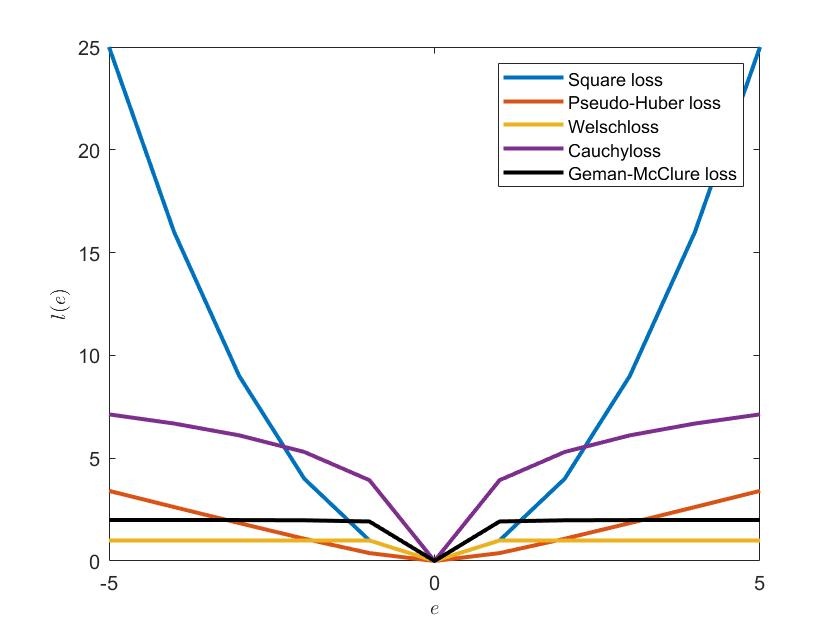
\includegraphics[scale=0.3]{CompareLoss.jpg}
	\caption{نمایش برخی از توابع خطا}\label{lossFun}
\end{figure}

\section{پیچیدگی محاسباتی الگوریتم یادگیری پیشنهادی}
در این بخش پیچیدگی محاسباتی الگوریتم یادگیری توزیع‌شده پیشنهادی بر اساس تعداد ضرب‌ها و جمع‌های استفاده شده در رابطه به‌روزرسانی گره $k$ در هر تکرار $t$ مورد بحث قرار می‌گیرد. پیچیدگی محاسباتی به صورت تابعی از پارامترهای $M$ (مرتبه فیلتر یا طول بردار پارامترها) و $N$ (تعداد گره‌ها در شبکه) بیان می‌شود. تعداد عملیات استفاده شده در الگوریتم \lr{RDSGD} به فرم \lr{ATC} در جدول \ref{tableexample} لیست شده‌اند. پیچیدگی محاسباتی \lr{RDSGD} از مرتبه $O(NM)$ است.


\begin{table}
	\centering
	\caption{هزینه محاسباتی الگوریتم \lr{RDSGD} برای گره $k$ در هر تکرار  }\label{Compexity}
	\begin{tabular}{ccc}\hline
		\lr{Term} & \lr{Multiplication Op.} & \lr{Addition Op.} \\\hline
		$\sum_{l\in N_k}a_{lk} w_{l,t-1}$ & $NM$ & $(N-1)M$  \\\hline
		$S_t^{-1}$ & $2M^2+2M$ & $3M^2-1$ \\\hline
		$\mu S_t^{-1}\lambda\left(\sum_{l\in N_k}a_{lk} w_{l,t-1}\right)$ & $M^2$ & $(M-1)M$  \\\hline
		$w^T_{k,t}u_{k,t}$ & $M$ & $M-1$  \\\hline
		$e_k(t)=d_k(t)-w_{k,t-1}^T u_{k,t}$ & 0 & 1  \\\hline
		$e_k(t)u_{k,t}$& $M$ & 0  \\\hline
		$\sqrt{1+\left(\frac{e_k(t)}{\delta}\right)^2}$ & 3 & 1  \\\hline
		$\frac{e_k(t)u_{k,t}}{\sqrt{1+\left(\frac{e_k(t)}{\delta}\right)^2}}$ & $M$ & 0  \\\hline
		$\sum_{l\in N_k}a_{lk}\frac{e_k(t)u_{k,t}}{\sqrt{1+\left(\frac{e_k(t)}{\delta}\right)^2}}$ & $NM$ & $(N-1)M$  \\\hline
		$\mu S_t^{-1}\sum_{l\in N_k}a_{lk}\frac{e_k(t)\textbf{u}_{k,t}}{\sqrt{1+\left(\frac{e_k(t)}{\delta}\right)^2}}$ & $M^2$ & $(M-1)M$ \\\hline
		$w_{k,t}$  & 0 & $2M$   \\\hline
		\textbf{\lr{Total}}  & $2NM+4M^2$ & $2NM+5M^2$  \\
		\textbf{\lr{per iteration}} & $+5M+3$ & $-M$ \\\hline
	\end{tabular}
	\label{tableexample}
\end{table}

تعداد عملیات ضرب و جمع الگوریتم یادگیری \lr{DSGD} به ترتیب $2NM-4M^2-4M$ و $2NM+5M^2-M-1$ است. در حالی‌که $N>M$ باشد، پیچیدگی محاسباتی الگوریتم یادگیری \lr{DSGD} از مرتبه $O(NM)$ است. الگوریتم‌های \lr{DSGD} و \lr{RDSGD} از لحاظ مرتبه زمانی مشابه هستند و اختلاف تعداد عملیات ضرب و جمع آن‌ها اندک است که با توجه به مقاوم بودن و کارایی بالا الگوریتم یادگیری \lr{RDSGD} این اختلاف قابل چشم‌پوشی است. از آنجایی‌که رابطه به‌روزرسانی الگوریتم \lr{DRLS} در گام تطبیق برای هر گره در هر تکرار $t$ شامل عملیات ماتریسی از اندازه $M\times M$ می‌باشد، پیچیدگی محاسباتی آن از مرتبه $O(NM^2)$ است. بنابراین پیچیدگی محاسباتی الگوریتم یادگیری \lr{RDSGD} با مرتبه $O(NM)$ خیلی کمتر از پیچیدگی محاسباتی الگوریتم \lr{DRLS} است. درحالی‌که رفتار همگرایی \lr{RDSGD} در برابر نویز گاوسی و در محیط ایستا تقریبا مشابه‌ رفتار همگرایی \lr{DRLS} است اما در حضور نویزهای غیرگاوسی  و به خصوص در محیط‌های غیرایستا، \lr{RDSGD} بر الگوریتم یادگیری \lr{DRLS} غلبه می‌کند. 
تعداد عملیات ضرب مورد نیاز در الگوریتم‌های \lr{DLMS} و \lr{RDLMS} به ترتیب $2NM+M$ و $2NM+4M+3$ است. همچنین تعداد عملیات جمع آن‌ها به ترتیب $2NM-M$ و $2NM+1$ می‌باشد. علی‌رغم وجود اختلاف در تعداد عملیات محاسباتی الگوریتم‌های \lr{DLMS}،  \lr{RDLMS} و \lr{RDSGD}، به دلیل مقاوم بودن و کارایی \lr{RDSGD} این اختلاف قابل چشم‌پوشی است. در جدول \ref{CompareCompexity} پیچیدگی محاسباتی این الگوریتم‌ها به طور مختصر با هم مقایسه شده‌اند. 
\begin{table}
	\centering
	\caption{مقایسه پیچیدگی محاسباتی برخی از الگوریتم‌های تطبیقی انتشاری}\label{CompareCompexity}
	\begin{tabular}{|c@{\hspace{6mm}}|@{\hspace{9mm}}c@{\hspace{19mm}}
			|}
		\hline
		\lr{Computational Complexity} & \lr{Algorithm}   \\
		\hline
		$O(NM+M)$ & \lr{DLMS} \\
		\hline  
		$O(NM+M)$ & \lr{RDLMS} \\
		\hline 
		$O(NM^2)$ & \lr{DRLS} \\
		\hline
		$O(NM+M^2)$ & \lr{DSGD} \\
		\hline
		$O(NM+M^2)$ & \lr{RDSGD} \\
		\hline      
	\end{tabular}
\end{table}



\section{الگوریتم‌های مورد مقایسه در آزمایشات}
در این بخش الگوریتم‌ها و روش‌های ارائه شده توسط محققان دیگر که مشابه روش پیشنهادی بوده و در بخش ارزیابی با آن مقایسه شده‌اند، ذکر می‌شوند.

\subsection{الگوریتم‌های مورد مقایسه از جنبه روش‌های مختلف یادگیری تطبیقی توزیع‌شده }
به منظور بررسی کارایی و رفتار همگرایی الگوریتم یادگیری پیشنهادی، الگوریتم‌های یادگیری انتشاری مشابه ارائه شده در سایر تحقیقات از جمله  \lr{DLMS}، \lr{DRLS}، \lr{DMCC}، \lr{DLMF}، \lr{DSignLMS} و \lr{Robust DLMS} مورد مقایسه قرار داده شده‌اند. الگوریتم‌های \lr{DRLS}  \cite{Cat20082} و \lr{DLMS}  \cite{Lop2008} به ترتیب نسخه‌های توزیع‌شده انتشاری الگوریتم‌های \lr{RLS} و \lr{LMS} می‌باشند. الگوریتم انتشار معيار حداكثرسازي کورآنتروپی (\lr{DMCC}) \cite{MA2016} مبتنی بر مفاهیم تئوری اطلاعات است و از كرنل گوسي به دليل توانايي آن در رد كردن نمونه‌هاي آغشته به نويز غيرگوسي جهت مقاوم‌سازی رویکرد یادگیری استفاده شده است.

در الگوريتم توزیع‌شده انتشاری  \lr{DLMF} \cite{Park2014} ميانگين توان چهارم خطا در تابع هدف براي مقابله با نويز غيرگوسي به كارگرفته شده است. همچنين در الگوريتم انتشار \lr{Robust DLMS} \cite{Ashk} از تابع زيان شبه‌هابر به منظور مقابله با نویزهای گاوسی و غیرگاوسی استفاده شده است. الگوريتم انتشار علامت خطا \lr{DSignLMS} \cite{Ni2016}  یک الگوریتم یادگیری مبتني بر حداقل‌سازي ميانگين مربعات خطا است که از علامت خطا در تابع هدف استفاده می‌کند. 


\subsection{الگوریتم‌های مورد مقایسه از جنبه روش‌های مختلف همگام‌سازی}
به منظور ارزیابی رویکرد پیشنهادی از دیدگاه عملی علاوه‌بر استفاده از معیارهای کارایی آماری و سخت‌افزاری بر روی مجموعه داده‌های مصنوعی و واقعی، مقایسه آن با سایر رویکردهای پیشین از جمله  \lr{PSP}، \lr{Sync-Switch } و \lr{RNA Protocol } انجام می‌شود. 

همگام‌سازی در رویکرد \lr{PSP} \cite{Zhao2021} به روش احتمالی کنترل می‌شود، یعنی با نمونه‌برداری از گره‌های شرکت‌کننده در یادگیری درصدی از گره‌های سیستم که مرحله فعلی را به پایان رسانده‌اند را تخمین می‌زند. ایده اصلی روش \lr{PSP} این است که ما نیاز داریم فقط بخشی از گره‌ها نه همه آنها، در پروسه همگام‌سازی قرار بگیرند.  

روش  \lr{Sync-Switch} \cite{Syncswitch2021} مبتنی بر یک روش همگام‌سازی ترکیبی است و با بهره‌گیری از مزایای \lr{BSP} و \lr{ASP} با کاهش زمان یادگیری به طور هم‌زمان دقت همگرایی را حفظ می‌کند. فرایند یادگیری با مکانیزم همگام‌سازی \lr{BSP} آغاز می‌شود و در صورت برقراری یکی از شرایط 1) رسیدن به یک دقت همگرایی مشخص یا 2) به‌وجود آمدن کند‌کننده‌های گذرا،  مکانیزم همگام‌سازی به \lr{ASP} تغییر می‌کند. 

در روش \lr{RNA Protocol }   \cite{Mitigating2020} به منظور مقابله با مساله کندکننده‌ها در یادگیری توزیع‌شده از الگوریتم غیرمتمرکز \lr{AllReduce} جزئی برای مدیریت کلاسترهای ناهمگن بهره گرفته شده است. در این پروتکل، یک گره آغازگر به صورت تصادفی از بین گره‌ها انتخاب می‌شود. زمانیکه کار گره آغازگر کارش تمام شود، صرف نظر از اینکه سایر گره‌ها محاسبات‌شان را تمام کرده باشند یا خیر، عمل کاهش در کل شبکه انجام خواهد شد.

\section{نتایج آزمایش‌ها}
در این بخش نتایج بدست آمده از آزمایشات انجام شده بر روی داده‌های مصنوعی (داده‌های تولید شده به صورت تصادفی) و داده‌های واقعی، ارائه خواهد شد. ارزیابی و مقایسه‌ها در این فصل به دو بخش اصلی تقسیم می‌شود. بخش اول مربوط به ارزیابی الگوریتم‌های یادگیری تطبیقی انتشاری پیشنهادی می‌باشد و پس از آن در بخش دوم به ارزیابی رویکرد پیشنهادی پرداخته می‌شود.

\subsection{ارزیابی الگوریتم \lr{DSGD} در مساله شناسایی سیستم}
با انجام مجموعه‌ای از آزمایشات، کارایی و رفتار همگرایی الگوریتم یادگیری انتشاری \lr{DSGD} (الگوریتم \ref{Alg_DSGD}) را مورد ارزیابی و مقایسه با الگوریتم‌های یادگیری انتشاری دیگر قرار می‌دهیم. بدین منظور کلیه الگوریتم‌های یادگیری انتشاری به فرم \lr{ATC} در نظر گرفته شده‌اند و در این بخش آزمایشات بر روی  شبکه‌ای با 20 گره که توپولوژی آن در ابتدای هر شبیه‌سازی به طور تصادفی تولید می‌شود، انجام شده‌اند.

\begin{figure}
	\centering
	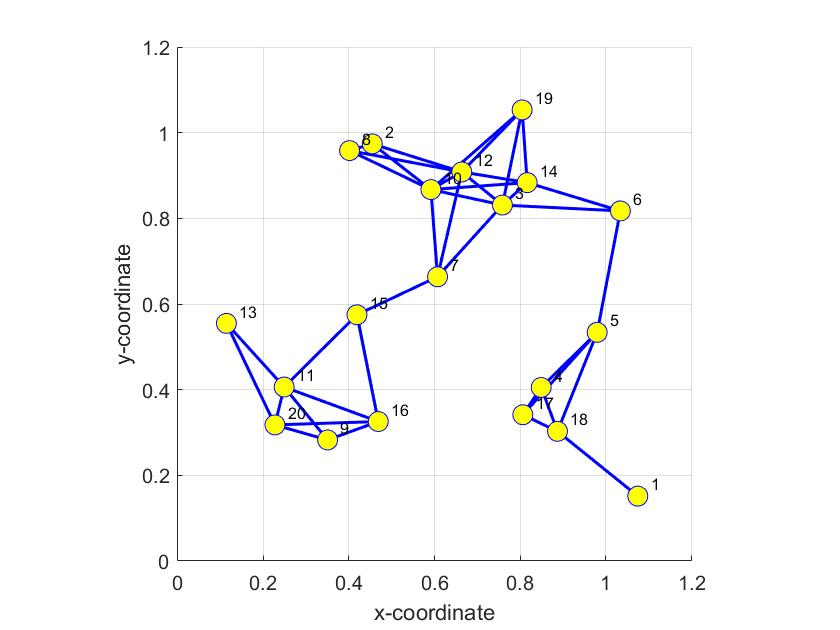
\includegraphics[scale=0.4]{topotogy.jpg}
	\caption{نمونه‌ای از توپولوژی شبکه تصادفی تولید شده با 20 گره}\label{Topology}
\end{figure}

پروفایل آماری شبکه در شکل \ref{Power} نشان می‌دهد که قدرت سیگنال و نویز گره‌ها در یک شبکه متفاوت است. الگوریتم \lr{DSGD} در \lr{MATLAB} پیاده‌سازی شده است و  عملکرد الگوریتم‌ها بر حسب میانگین انحراف مربع (\lr{MSD}) شبکه بر روی مساله شناسایی سیستم اندازه‌گیری شده است که به صورت زیر تعریف می‌شود:
\begin{equation}\label{MSD}
	MSD^{network}(t)=\frac{1}{N}\sum_{k=1}^{N}E||w_o-w_{k,t}||^2
\end{equation}
مساله شناسایی سیستم در واقع علم ساخت مدل‌های ریاضی سیستم‌ها از روی داده‌های ورودی-خروجی است که در دهه‌های گذشته \cite{Sam2013} توجه زیادی را به خود جلب کرده است. شمای کلی یک گره در یک شبکه تطبیقی توزیع‌شده برای کاربرد شناسایی سیستم در شکل \ref{p13} در فصل \ref{ProposedApproach} نشان داده شده است. 
\begin{figure}
	\centering
	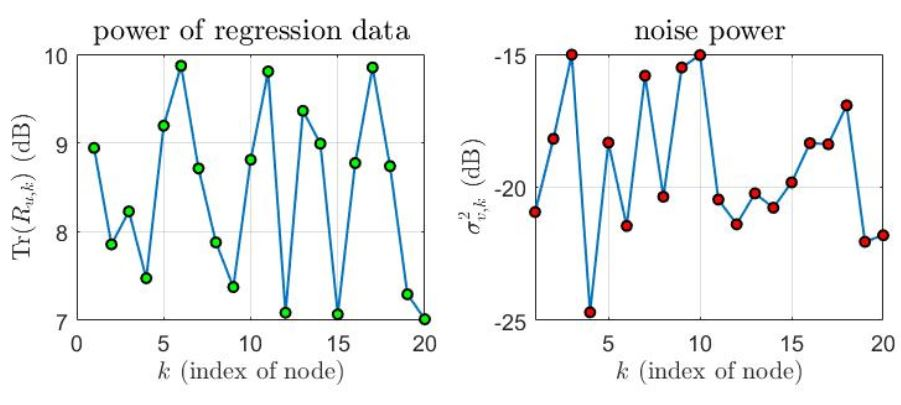
\includegraphics[scale=0.8]{regressor_noise_power__.jpg}
	\caption{واریانس‌های نویز و ردیابی کوواریانس‌های رگرسیون برای 20 گره}\label{Power}
\end{figure}

 در آزمایشات انجام شده اندازه گام (پارامتر نرخ یادگیری) به طور پیش‌فرض برای تمام الگوریتم‌ها $\mu=0.03$ تنظیم شده است؛ اگر برای الگوریتمی مقداری غیر از این باشد، حتما ذکر خواهد شد. همان‌طور که قبلا اشاره شد، ماتریس $S_t$ تاثیر قابل توجهی در تسریع نرخ همگرایی الگوریتم دارد. به منظور بررسی تاثیر آن بر نرخ همگرایی، دو حالت ثابت و متغیر را برای ماتریس $S_t$ در نظر می‌گیریم. در اولین حالت ماتریس $S_t=S$ را با ماتریس همانی از سایز $M\times M$ مقداردهی و نسخه ثابتی از الگوریتم $DiffusionSGD$ به نام $DSGD$ معرفی می‌شود. در حالت دیگر، ماتریس $S_t$ با هر نمونه داده ورودی جدید با زمان تغییر می‌کند. نسخه متغیر الگوریتم $DiffusionSGD$ به نام $DRSGD$ معرفی می‌شود. شکل \ref{Com_DSGD_DRSGD} منحنی‌های یادگیری سه الگوریتم، $SGD$ ساده بدون هیچ استراتژی انتشار و دو نسخه ثابت و متغیر الگوریتم $DiffusionSGD$ را بر اساس معیار $MSD$ مورد مقایسه قرار می‌دهد. در این آزمایش پارامترهای $\mu=0.03$, $M=5$, $T=500$ است و نتایج از میانگین 20 اجرای مستقل حاصل شده‌اند. 
 
 نتایج شبیه‌سازی تأثیر استراتژی‌انتشار و مقدار ماتریس $S_t$ را بر نرخ همگرایی نشان می‌دهد و به وضوح بیان می‌کند که روش \lr{DRSGD} سریع‌تر از دو روش دیگر همگرا می‌شود. در اجرای روش \lr{DRSGD}، از ایده محاسبه $R^{-1}$ در الگوریتم \lr{RLS} برای تنظیم $S_t$ در هر تکرار $t$ استفاده کردیم. این روش از توانایی بیشتری در استخراج اطلاعات مفید از سیگنال‌های نویزدار برخوردار است.
 
 \begin{figure}
 	\centering
 	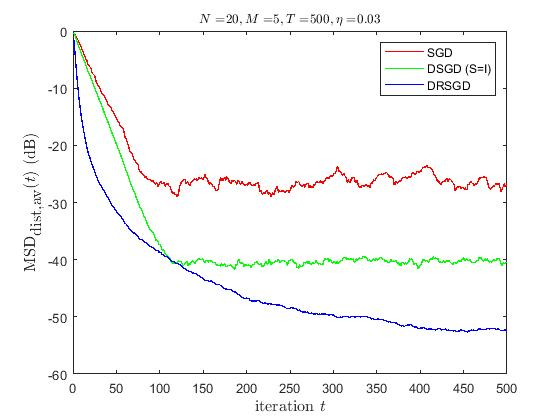
\includegraphics[scale=0.6]{Compare_DSGDandDRSGD_Gaussiannoise_F.jpg}
 	\caption{مقایسه الگوریتم‌های \lr{SGD} و \lr{DSGD} و \lr{ِDRSGD} با 500 تکرار و $M=5$ }\label{Com_DSGD_DRSGD}
 \end{figure}


یکی دیگر از پارامترهای موثر بر عملکرد و نرخ همگرایی الگوریتم\lr{DSGD} اندازه گام $\mu_t=\mu$ است. شکل \ref{DifferentMu} نتایج اعمال شش مقدار متفاوت $\mu$ را در الگوریتم \lr{DSGD} نشان می‌دهد. بر اساس نتایج ارائه شده، برای تضمین همگرایی سریع‌تر، مقدار $\mu$ نباید خیلی کوچک باشد و بهترین همگرایی زمان رخ می‌دهد که مقدار $\mu=0.03$ تنظیم شود.

\begin{figure}
	\centering
	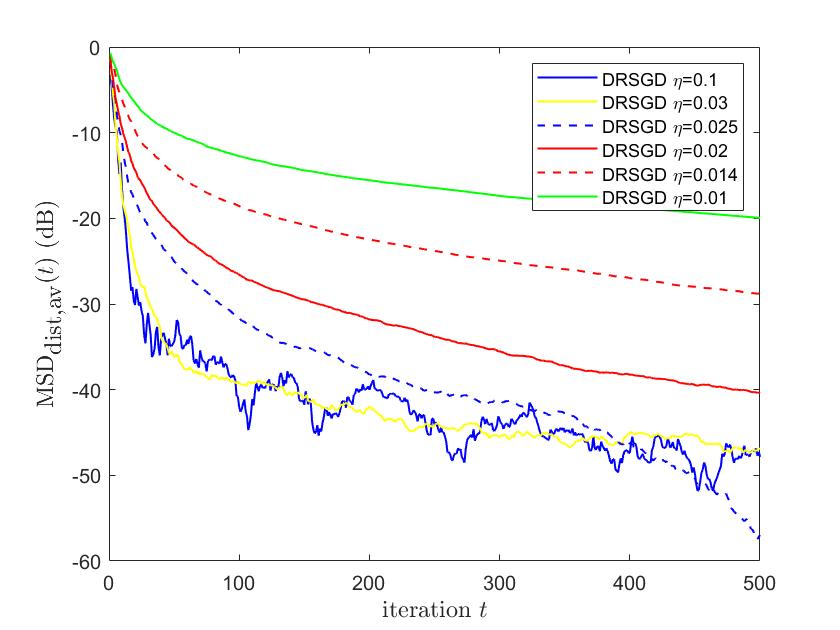
\includegraphics[width=5in]{Dif_eta.jpg}
	\caption{\lr{MSD} شبکه گذرا الگوریتم \lr{DSGD} با مقادیر  متفاوت اندازه گام در 500 تکرار و $M=5$}\label{DifferentMu}
\end{figure}

در آزمایش بعدی، از سنجه جدید اختلاف همگرایی وزنی \ref{DeltaW} برای بررسی همگرایی الگوریتم \lr{DSGD} استفاده شده است. شکل \ref{Delta_w} رفتار الگوریتم را بر اساس معیار اختلاف همگرایی وزنی $\Delta(w_{k,t},w_{k,t-1},w)$ در تکرارهای مختلف نشان می‌دهد. همان‌طور که دیده می‌شود، معیار $\Delta(w_{k,t},w_{k,t-1},w)$ در طول زمان روند کاهشی دارد و این بدین معناست که بردار تخمین‌زده شده در تکرار $t$ ،$w_t$، به بردار وزن دلخواه $w$ نزدیکتر از بردار تخمین‌زده شده در تکرار قبلی $w_{t-1}$ است.

\begin{figure}
	\centering
	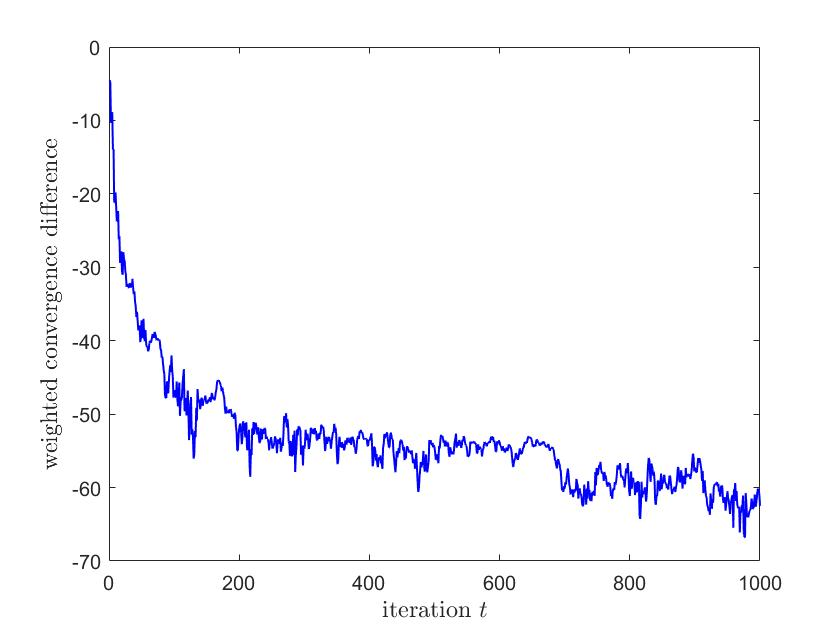
\includegraphics[scale=0.4]{deltaW_1000Sample_new.jpg}
	\caption{منحنی کارایی الگوریتم پیشنهادی بر اساس معیار اختلاف همگرایی وزنی در 1000 تکرار اول با طول بردار وزن 5}\label{Delta_w}
\end{figure}

در آزمایش بعدی، تأثیر توپولوژی شبکه بر عملکرد روش \lr{DSGD} بر اساس معیار اختلاف همگرایی وزنی، $\Delta(w_{k,t},w_{k,t-1},w)$ بررسی شده است. ما روش \lr{DSGD} را روی چهار توپولوژی مختلف شبکه با 20 گره اعمال کرده و منحنی‌های عملکرد آن را در 100 تکرار اول نشان داده‌ایم. چهار توپولوژی‌ مختلف از یک شبکه با 20 گره را می‌توان در شکل \ref{fourTop} مشاهده کرد. بر اساس نتایج نشان داده شده در شکل \ref{DifferentTop}، می‌توان نتیجه گرفت که معیار $\Delta(w_{k,t},w_{k,t-1},w)$ در طول فرایند یادگیری الگوریتم \lr{DSGD} در تمام توپولوژی‌های شبکه روند کاهشی دارد. این موضوع نشان می‌دهد که بردار وزن $w_t$ در طول زمان به بردار وزن بهینه $w$ نزدیکتر می‌شود.

\begin{figure}
	\centering
	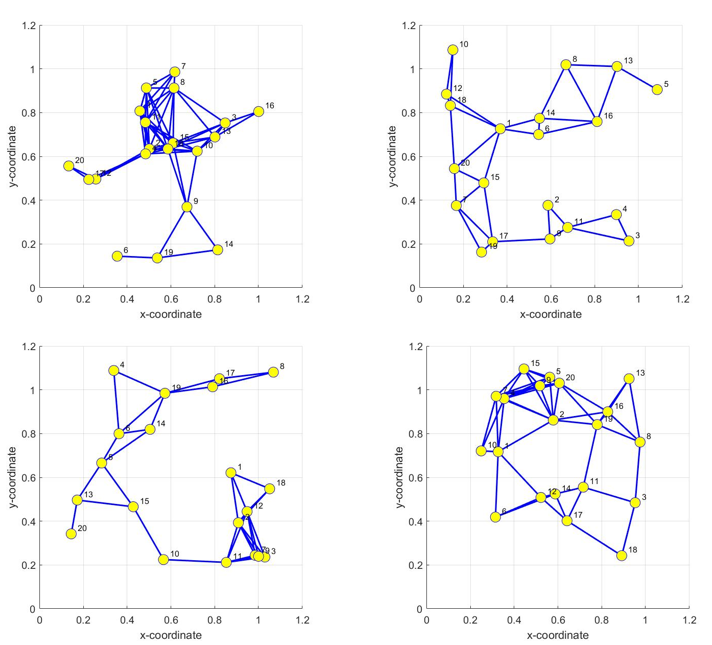
\includegraphics[scale=1]{Four_Topo.PNG}
	\caption{توپولوژی‌های مختلف شبکه}\label{fourTop}
\end{figure}


\begin{figure}
	\centering
	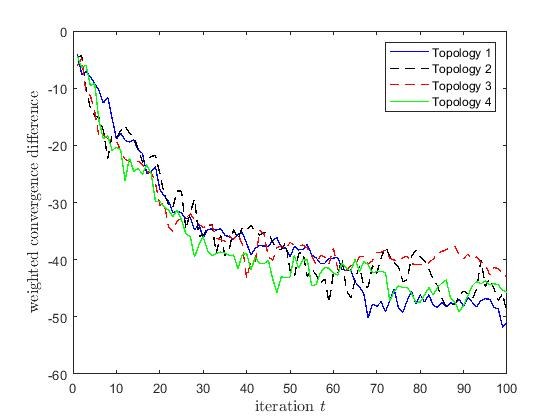
\includegraphics[scale=0.55]{Dif_Topo.jpg}
	\caption{منحنی عملکرد الگوریتم پیشنهادی بر روی شبکه هایی با توپولوژی متفاوت }\label{DifferentTop}
\end{figure}

عملکرد و سرعت همگرایی الگوریتم پیشنهادی در حالت متغیر \lr{DRSGD} را با الگوریتم‌های \lr{DLMS} معمولی، \lr{DRLS} معمولی، الگوریتم‌های \lr{DMCC} و \lr{ِDLMF} در فرم \lr{ATC} مقایسه کرده‌ایم. در این آزمایش، فرایند یادگیری با 500 و 1000 تکرار مورد بررسی قرار گرفته است. به منظور داشتن نرخ همگرایی اولیه یکسان در تمام الگوریتم‌های مورد مقایسه، اندازه گام $\mu=0.03$ در نظر گرفته شده است. شکل \ref{Com_DRSGD_LMS_RLS} منحنی مقادیر \lr{MSD} برای الگوریتم‌های مورد مقایسه در محیطی آغشته به نویز گاوسی با 500 تکرار فرایند یادگیری را نشان می‌دهد. 

همانطور که مشاهده می‌شود، نرخ همگرایی الگوریتم پیشنهادی \lr{DRSGD} سریع‌تر از الگوریتم‌های \lr{DLMS}، \lr{DMCC} و \lr{DLMF} می‌باشد، در حالی‌که نرخ همگرایی \lr{DRSGD} کمی کمتر از \lr{DRLS} است. با افزایش تعداد تکرارها از 500 به 1000 تکرار در شکل \ref{n700}، مشاهده می‌شود که\lr{DRSGD} به منحنی \lr{MSD} بهتری دست می‌یابد و تقریبا همانند الگوریتم \lr{DRLS} رفتار می‌کند. این اختلاف ناچیز در مقایر همگرا شده را می‌توان در مقابل اختلاف بین پیچیدگی محاسباتی \lr{DRSGD} و \lr{DRLS} نادیده گرفت. پیچیدگی محاسباتی الگوریتم‌های انتشار بر حسب تعداد عملیات ضرب و جمع در هر تکرار برای هر گره برحسب پارامترهای $M$ (طول بردار وزن یا اندازه فیلتر) و $N$ (تعداد کل گره‌های شبکه) مورد بحث قرار می‌گیرد. از آنجایی که \lr{DRLS} شامل عملیات ماتریسی با اندازه $M*M$ در مرحله انطباق در هر تکرار $t$ برای هر گره است، پیچیدگی محاسباتی آن از مرتبه $O(NM^2)$ است، که در آن $N$ عدد است. همانطور که انتظار می‌رود، از آنجایی که $N>M$، پیچیدگی محاسباتی الگوریتم پیشنهادی \lr{DRSGD}، با مرتبه $O(NM)$، بسیار کمتر از \lr{DRLS} است. علاوه‌بر این، \lr{DRLS} فقط برای یادگیری آنلاین مناسب است، در حالی‌که \lr{DRSGD} برای یادگیری آنلاین و آفلاین کاربرد دارد. از سوی دیگر، \lr{DRLS} به ترتیب ورود داده‌ها حساس است اما \lr{DRSGD} به این مورد حساس نیست.

\begin{figure}
	\centering
	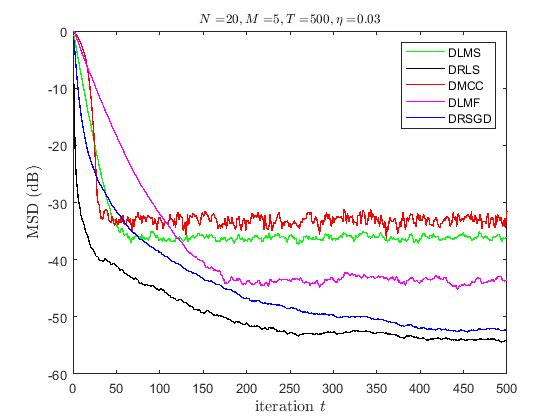
\includegraphics[scale=0.5]{Compare5Algorithm.jpg}
	\caption{مقایسه بین الگوریتم پیشنهادی و الگوریتم‌های انتشار بر روی \lr{MSD} با 500 تکرار و طول فیلتر 5}\label{Com_DRSGD_LMS_RLS}
\end{figure}


\begin{figure}
	\centering
	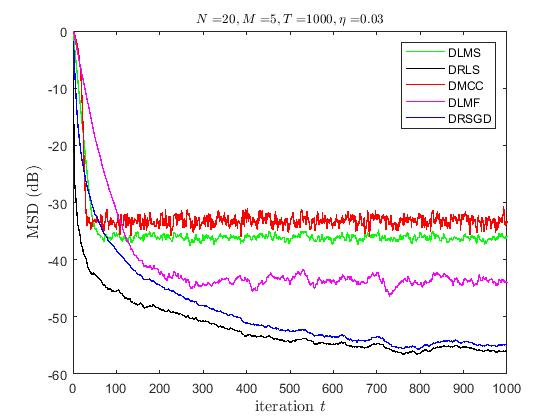
\includegraphics[scale=0.5]{1000.jpg}
	\caption{مقایسه بین الگوریتم پیشنهادی و الگوریتم‌های انتشار بر روی \lr{MSD} با 1000 تکرار و طول فیلتر 5}\label{n700}
\end{figure}

\subsection{ارزیابی الگوریتم \lr{RDSGD} در محیط ایستا}
استفاده از توابع زیان مقاوم در برابر نویزهای مختلف محیطی سبب افزایش مقاومت روش الگوریتم یادگیری توزیع‌شده می‌شود. تابع زیان مربع خطا  تنها در برابر نویزهای گاوسی مقاوم است اما در محیط‌های آغشته به نویزهای غیرگاوسی عملکرد ضعیفی دارد و در اکثر مواقع واگرا می‌شود. توابع زیانی مانند شبه‌هابر، کورآنتروپی و ... نسبت به نویزهای غیرگاوسی مقاوم می‌باشند. 

در این بخش، نتایج آزمایش‌ها برای نشان دادن عملکرد الگوریتم مقاوم \lr{RDSGD} در حل مسائل شناسایی سیستم و پیش‌بینی و همچنین بررسی تأثیر پارامترهای مختلف بر عملکرد تخمین آن ارائه می‌شوند. الگوریتم \lr{RDSGD} با الگوریتم‌های انتشار مرسوم و الگوریتم‌های انتشار قوی از نظر مقاوم بودن در محیط‌های ایستا و غیرایستا مورد مقایسه قرار خواهد گرفت. این مقایسه‌ها در حضور نویزهای گاوسی و غیر گاوسی ارزیابی می‌شوند. در این رساله، نویزهای غیر گاوسی با توزیع آلفا پایدار و گاوسی مخلوط مدل‌سازی می‌شوند. نویز آلفا پایدار به صورت $V_{\alpha-stable}(1.3, 0, 1.2, 0)$ تنظیم شده است. این مجموعه از آزمایش‌ها نیز بر روی شبکه‌ای با 20 گره و طول بردار وزن $M=5$ انجام شده‌اند. نتایج گزارش‌شده به صورت میانگین 20 آزمایش مستقل می‌باشند که عملکرد الگوریتم‌ها را برحسب معیار \lr{MSD} شبکه اندازه‌گیری می‌کنند.


برای ارزیابی عملکرد، رفتار یادگیری الگوریتم \lr{RDSGD} از نظر مقاوم بودن در برابر نویز برای مساله شناسایی سیستم با سایر الگوریتم‌ها مانند \lr{DMCC} \cite{MA2016}، \lr{DLMS} \cite{Lop2008}، \lr{DRLS} \cite{Cat20082}،\lr{DSGD}، \lr{DLMF} \cite{DLMF2017}، \lr{DsignLMS} \cite{DsignLMS2016} و \lr{RDLMS} مقایسه می‌شود. در این بخش، این مقایسه‌ها در محیطی ایستا و تحت نویز گاوسی و نویزهای غیرگاوسی مورد ارزیابی قرار می‌گیرند. یک محیط ایستا به مدل استاتیک سیستم در زمان اشاره می‌کند. اندازه گام $\mu$ برای \lr{DLMF} $0.25$، برای \lr{DLMS}، \lr{DRLS}، \lr{DSGD}، \lr{RDSGD} $0.03$، برای \lr{DMCC} $0.05$، برای \lr{DsignLMS} $0.09$  و برای \lr{RDLMS} $0.07$ تنظیم شده است. 
در آزمایش اول، منحنی عملکرد الگوریتم‌ها در محیط آغشته به نویز آلفا پایدار در شکل \ref{StAlpha} نشان داده شده‌اند.
\begin{figure}[htbp]  \centering{
		\subfigure[]{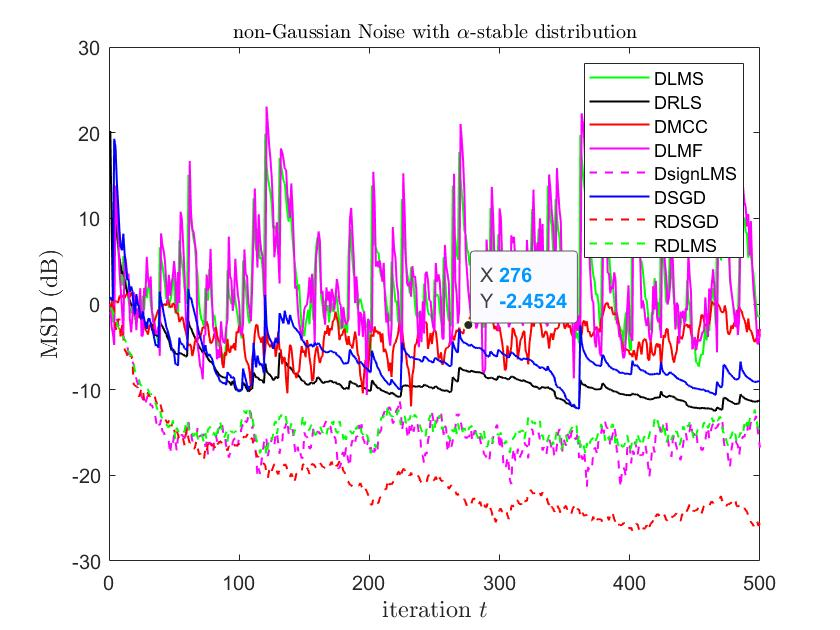
\includegraphics[width=10 cm,height=7 cm]{AllCom_AlphaSt8.png}\label{StAlpha}}
		\subfigure[]{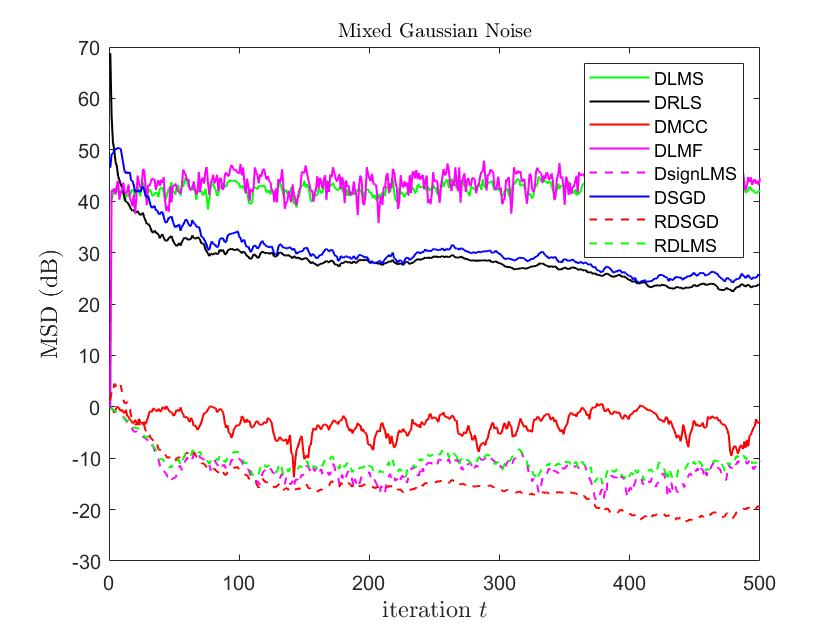
\includegraphics[width=10 cm,height=7 cm]{AllCom_MixGau_St8.png}\label{StMixGassian}}
		\\
		\subfigure[]{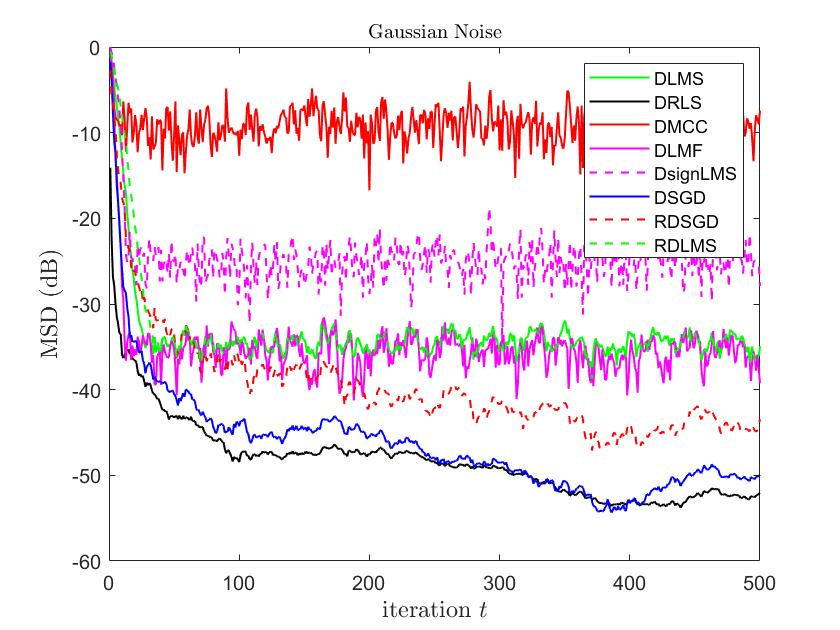
\includegraphics[width=10 cm,height=7 cm]{AllCom_Gau_St8.png}\label{StGaussian}}
	}
	\caption[]{مقایسه رفتار همگرایی الگوریتم‌ها در محیط ایستا. الف) نویز الفا پایدار با $SNR=-20 dB$
	ب) نویز گاوسی مخلوط با $SNR=-50 dB$
ج) نویز گاوسی با $SNR=20 dB$} 
	\label{AllStationary}
\end{figure}
همانطور که مشاهده می‌شود، \lr{DLMS}، \lr{DRLS}، \lr{DLMF}، \lr{DMCC} و \lr{DSGD} در حضور نویز پایدار $\alpha$ واگرا هستند و \lr{RDSGD}، \lr{RDLMS} و \lr{DisignLMS} نسبت به سایر الگوریتم‌ها در حالت پایدار با خطای کمتری همگرا می‌شوند. با این حال \lr{RDSGD} از سایر الگوریتم‌ها بهتر عمل می‌کند. نتایج ارائه شده در شکل \ref{StAlpha} نشان می‌دهند که الگوریتم پیشنهادی در برابر نویز پایدار $\alpha$ مقاوم است و سریع‌تر از سایر الگوریتم‌ها همگرا می‌شود.

شکل \ref{StMixGassian} منحنی رفتاری الگوریتم‌ها را بر حسب معیار \lr{MSD} در حضور نویز گاوسی مخلوط با $SNR=-50dB$ نشان می‌دهد. این نویز توسط  $GMM(\mu_{G1},\mu_{G2},\sigma)$ مدل‌سازی شده است. اندازه گام برای \lr{DMCC} $0.3$، برای \lr{DsignLMS} $0.09$، برای \lr{DLMF} $0.25$، برای \lr{RDLMS} $0.07$، برای \lr{DLMS}، \lr{DRLS}، \lr{DSGD} و \lr{RDSGD} $0.05$ تنظیم شده است. همانطور که در شکل \ref{StMixGassian}، برای نویز گاوسی مخلوط با $SNR=-50 dB$ و توزیع $GMM(\mu_{G1}=1,\mu_{G2}=300،\sigma=1)$ مشاهده می‌شود،  الگوریتم‌های \lr{DLMS} و \lr{DLMF} واگرا شده‌اند. \lr{RDSGD}، \lr{RDLMS}، \lr{DsignLMS} و \lr{DMCC} از الگوریتم‌های دیگر بهتر عمل می‌کنند در حالی‌که در حالت پایدار، \lr{RDSGD} بهتر از \lr{RDLMS}، \lr{DsignLMS} و \lr{DMCC} است و سریعتر به مقدار خطای کمتری همگرا می‌شود. بر این اساس، می‌توان نتیجه گرفت که \lr{RDSGD} از همه الگوریتم‌های رقیب مقاوم‌تر است و بهتر عمل می‌کند.

الگوریتم‌های انتشار مقاوم بسیاری پیشنهاد شده‌اند، اما عملکرد آنها برای مقابله با نویزهای گاوسی خوب نیست. اندازه گام $\mu$ برای \lr{DLMF} $0.15$، برای \lr{DLMF}، $0.05$ برای \lr{DLMS}، \lr{DRLS}، \lr{DSGD}، \lr{RDSGD}، $0.2$ برای \lr{DMCC}، $ 0.03$ برای \lr{DsignLMS} و $ 0.07$ برای \lr{RDLMS} تنظیم شده است. شکل \ref{StGaussian} نشان می‌دهد که \lr{DMCC} و \lr{DsignLMS} که برای نویزهای غیر گاوسی قوی هستند، اما در برابر نویز گاوسی خوب عمل نمی‌کنند. همانطور که مشاهده می‌شود، \lr{DRLS}، \lr{RDSGD} و \lr{DSGD} از \lr{DLMF}، \lr{DLMS} و \lr{RDLMS} بهتر عمل می‌کنند. \lr{DRLS} و \lr{DSGD} رفتار همگرایی تقریبا مشابهی دارند. با این حال، می‌توان نتیجه گرفت که الگوریتم پیشنهادی می‌تواند نویزهای گاوسی و غیر گاوسی را در محیط ایستا مدیریت کند.

اندازه گام $\mu$ پارامتر بسیار موثری بر کارایی و نرخ همگرایی الگوریتم \lr{RDSGD} است. در شکل \ref{mu_alpha} منحنی‌های کارایی \lr{RDSGD} به ازای مقادیر مختلف $\mu$ نشان داده شده است. از نتایج ارائه شده می‌توان نتیجه گرفت که مقدار $\mu$ نباید خیلی بزرگ یا خیلی کوچک باشد تا عملکرد و همگرایی سریع الگوریتم تضمین شود. بر اساس نتایج ارائه شده در شکل \ref{mu_alpha}، برای مساله شناسایی سیستم و در حضور نویز آلفا پایدار، مقدار مناسب $\mu$ برای \lr{RDSGD} $0.05$ است.

\begin{figure}[ht]
	\centering
	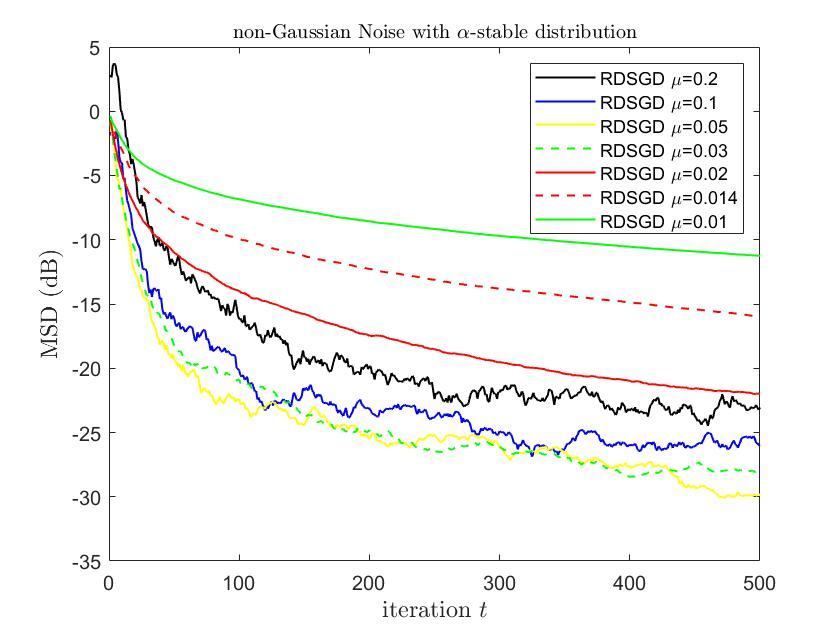
\includegraphics[scale=0.3]{mu_alpha_5Iter.jpg} 
	\caption{منحنی \lr{MSD} الگوریتم \lr{RDSGD} به ازای مقادیر مختلف اندازه گام در حضور نویز آلفا پایدار با $SNR=-20 dB$}
	\label{mu_alpha}
\end{figure}

شکل \ref{SSP_Sta} عملکرد گره‌های شبکه را در حالت پایدار با کمک منحنی \lr{MSD} در حضور نویزهای گاوسی، گاوسی آمیخته و نویز الفا پایدار در محیط ایستا نشان می‌دهد. همان طور که دیده می‌شود، گره‌ها در حالت پایدار به مقادیر خطای تقریبا نزدیک بهم همگرا می‌شوند. شکل \ref{SSP_1} نیز عملکرد گره‌های شبکه در حالت پایدار برای تعدادی از الگوریتم‌ها را مورد مقایسه قرار می‌دهد. 

\begin{figure}[ht]
	\centering
	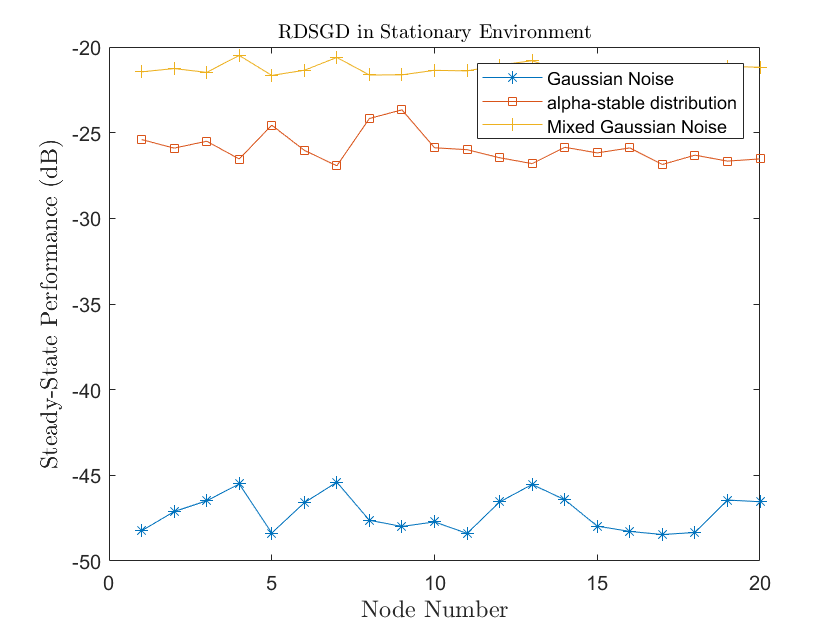
\includegraphics[scale=0.4]{SSP_Noise_Stationary_1.png} 
	\caption{منحنی \lr{MSD} عملکرد گره‌های مختلف در یک شبکه  با 20 گره در حالت پایدار}
	\label{SSP_Sta}
\end{figure}

\begin{figure}[htbp]  \centering{
		\subfigure[]{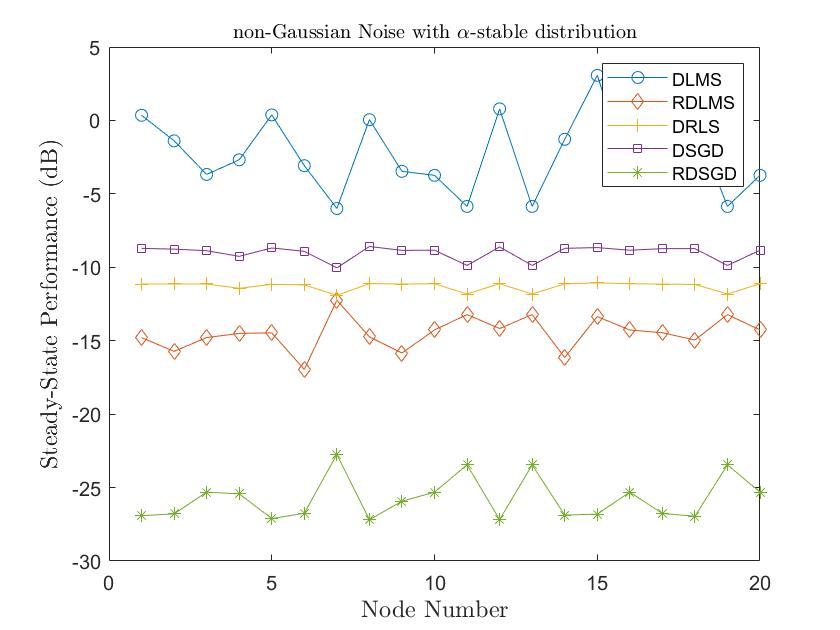
\includegraphics[width=10 cm,height=7 cm]{AlphaStable_SSP_.jpg}\label{SSP-alpha_}}
		\subfigure[]{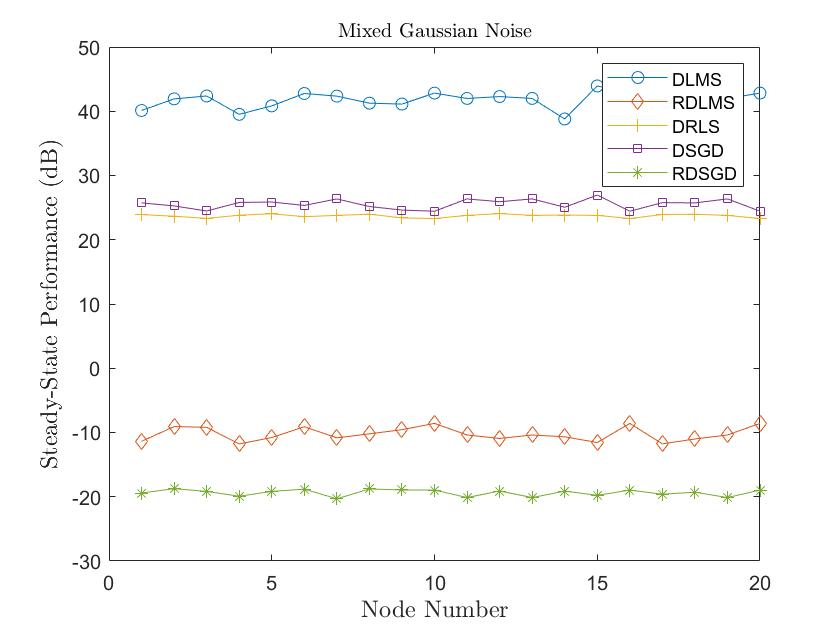
\includegraphics[width=10 cm,height=7 cm]{MixGaussian_SSP_.jpg}\label{SSP-mix_}}
		\\
		\subfigure[]{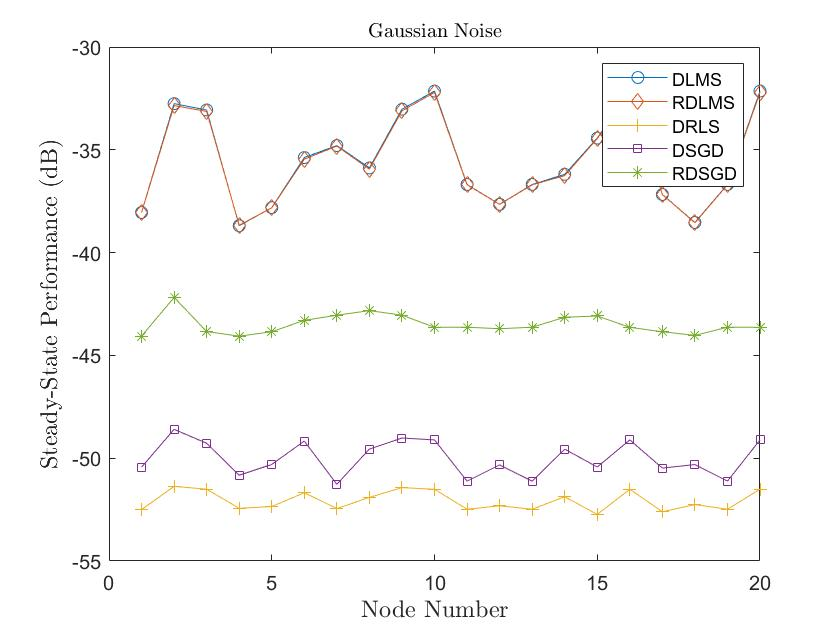
\includegraphics[width=10 cm,height=7 cm]{Gaussian_SSP_.jpg}\label{SSP-gaussian_}}
	}
	\caption[]{مقایسه رفتار همگرایی  گره‌ها در حالت پایدار  برای تعدادی از الگوریتم‌ها در محیط ایستا. الف) نویز الفا پایدار با $SNR=-30 dB$
		ب) نویز گاوسی مخلوط با $SNR=-50 dB$
		ج) نویز گاوسی با $SNR=20 dB$} 
	\label{SSP_1}
\end{figure}





\subsection{ارزیابی الگوریتم \lr{RDSGD} در محیط‌ غیرایستا}
محیط غیرایستا به حالتی اشاره دارد که  مدل سیستم در طول زمان تغییر می‌کند. آموزش الگوریتم‌های انتشار با عملکرد خوب در محیط‌های غیرایستا دشوار است و بسیاری از این الگوریتم‌ها توانایی ارائه نتایج قابل قبولی در محیط‌های غیرایستا ندارند. در ادامه، عملکرد \lr{RDSGD} در محیط غیرایستا مدل‌شده با \ref{Track} و در شرایطی مشابه با آزمایشات محیط ایستا بررسی می‌شود.

شکل \ref{non_1} رفتار همگرایی الگوریتم‌ها را در مقابل نویزهای گاوسی، گاوسی مخلوط و نویز الفا پایدار در محیط غیرایستا نشان می‌دهد. در حضور نویزهای غیرگاوسی، الگوریتم پیشنهادی قادر است تاثیر نمونه‌های اغشته به نویز را کاهش دهد. به عبارت دیگر، حساسیت کمتری به نویز دارد. همان‌طور که در شکل \ref{non-alpha} و \ref{non-mix} دیده می‌شود، الگوریتم \lr{RDSGD} در محیط غیرایستا به سایر الگوریتم‌های رقیب غلبه می‌کند. شکل \ref{non-gaussian} نشان می‌دهد که در حضور نویز گاوسی نیز الگوریتم پیشنهادی بر الگوریتم‌های \lr{DLMS}، \lr{DRLS}، \lr{DMCC}، \lr{DLMF}، \lr{DsignLMS} غلبه می‌کند و این در حالی است که الگوریتم \lr{DSGD} در حالت پایدار بهتر از \lr{RDSGD} عمل می‌کند و به سایر الگوریتم‌ها هم غلبه کرده است. 

\begin{figure}[htbp]  \centering{
		\subfigure[]{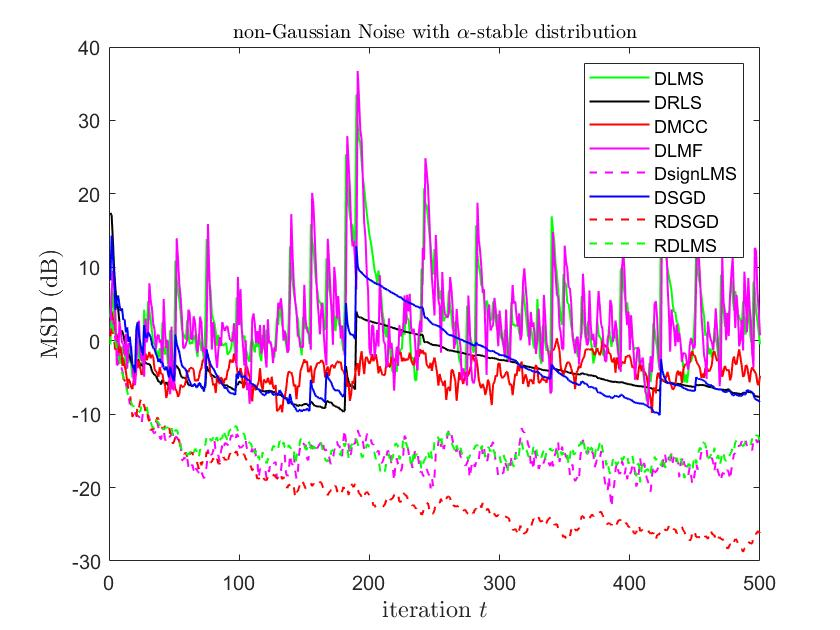
\includegraphics[width=10 cm,height=7 cm]{AllCom_AlphaNon8.png}\label{non-alpha}}
		\subfigure[]{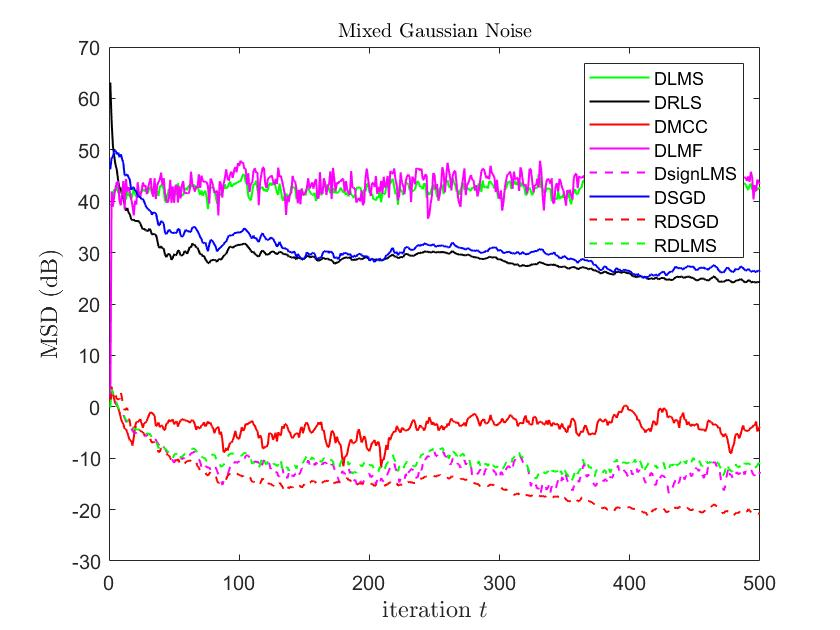
\includegraphics[width=10 cm,height=7 cm]{AllCom_MixGau_Non8.png}\label{non-mix}}
		\\
		\subfigure[]{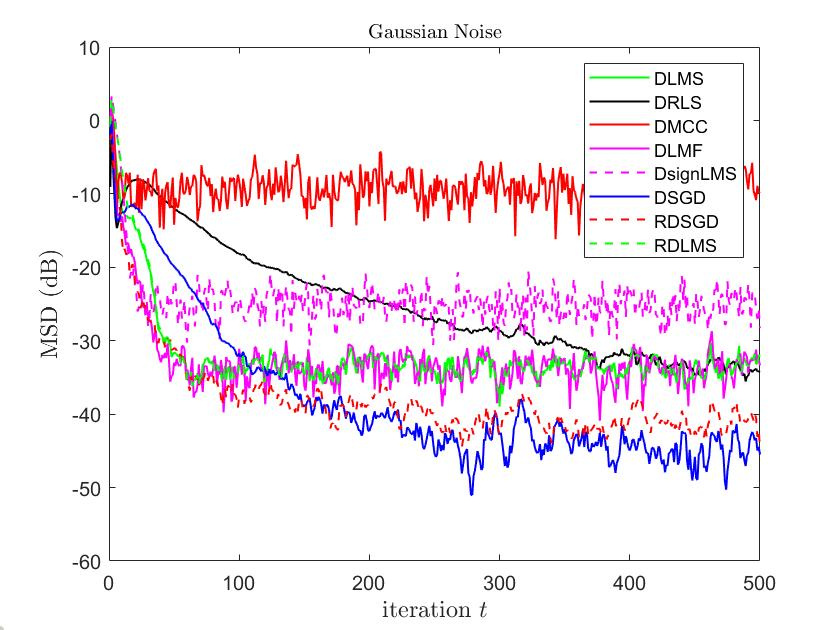
\includegraphics[width=10 cm,height=7 cm]{AllCom_Gau_Non8.png}\label{non-gaussian}}
	}
	\caption[]{مقایسه رفتار همگرایی الگوریتم‌ها در محیط غیرایستا. الف) نویز الفا پایدار با $SNR=-30 dB$
		ب) نویز گاوسی مخلوط با $SNR=-50 dB$
		ج) نویز گاوسی با $SNR=20 dB$} 
	\label{non_1}
\end{figure}

در آزمایشی دیگر، تاثیر توابع زیان مختلف بر رفتار همگرایی و میزان خطا در حالت پایدار الگوریتم \lr{DSGD} در محیط غیرایستا مورد بررسی و مطالعه قرار گرفته است. توابع زیان استفاده شده در این آزمایش شامل مربع خطا، شبه‌هابر، تابع زیان \lr{Cauchy} \cite{CauchyLoss}، \lr{Geman-McClure} \cite{GemanLoss}، \lr{Welsch} \cite{WelschLoss} می‌باشند که الگوریتم‌های متناظر با این توابع زیان به ترتیب \lr{DSGD}، \lr{RDSGD}، \lr{GemanDSGD}، \lr{CauchyDSGD} و \lr{WelschDSGD} نام‌گذاری شده‌اند. شکل \ref{OtherLoss} رفتار همگرایی این الگوریتم‌ها را در مقابل نویزهای گاوسی، گاوسی مخلوط و نویز الفا پایدار نشان می‌دهد. همان‌طور که در شکل \ref{OtherLossAlpha} دیده می‌شود، \lr{RDSGD} تا تکرار 600 به تمام الگوریتم‌ها غلبه کرده است، اما از آن به بعد \lr{RDSGD} و \lr{CauchyDSGD} تقریبا مشابه رفتار می‌کنند. 

همان‌طور که در شکل \ref{OtherLossMixGaussian} نشان داده است، در محیط آغشته به نویز گاوسی مخلوط، الگوریتم پیشنهادی  \lr{RDSGD} از همه الگوریتم‌ها بهتر عمل می‌کند و سریع‌تر از سایر الگوریتم‌ها به خطای کمتر در حالت پایدار همگرا می‌شود. شکل \ref{OtherLossGaussian} نشان می‌دهد که همه الگوریتم‌ها در برابر نویز گاوسی در محیط غیرایستا تقریباً یکسان عمل می‌کنند. با توجه به رفتار همگرایی الگوریتم‌ها در برابر سه نویز مورد بررسی، تابع زیان شبه‌هابر در مقایسه با سایر توابع زیان انتخاب مناسب‌تری است.

\begin{figure}[htbp]  \centering{
		\subfigure[]{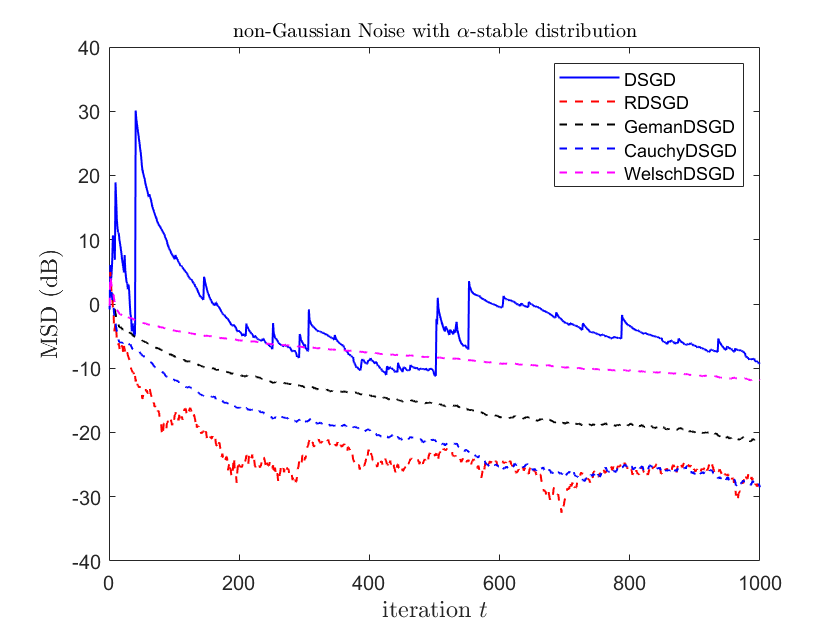
\includegraphics[width=9 cm,height=7 cm]{ComLossAlpha_non8.png}\label{OtherLossAlpha}}
		\subfigure[]{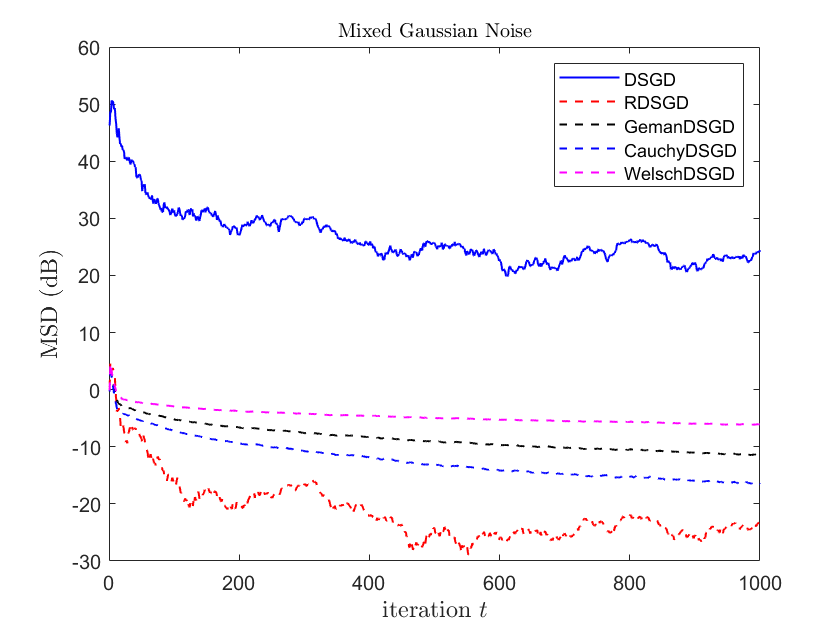
\includegraphics[width=9 cm,height=7 cm]{ComLossMixGau_non8.png}\label{OtherLossMixGaussian}}
		\\
		\subfigure[]{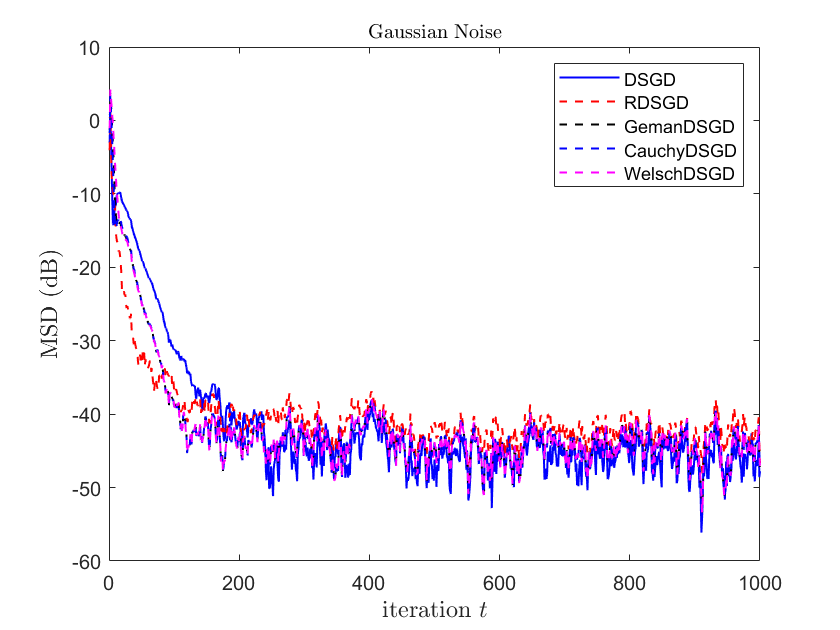
\includegraphics[width=9 cm,height=7 cm]{ComLossGau_non8.png}\label{OtherLossGaussian}}
	}
	\caption[]{تأثیر توابع زیان مختلف بر رفتار همگرایی الگوریتم \lr{DSGD} در محیط غیرایستا. الف) نویز الفا پایدار
		ب) نویز گاوسی مخلوط
		ج) نویز گاوسی} 
	\label{OtherLoss}
\end{figure}

شکل \ref{SSP_nonSta} عملکرد گره‌های شبکه را در حالت پایدار با کمک منحنی \lr{MSD} در حضور نویزهای گاوسی، گاوسی آمیخته و نویز الفا پایدار در یک محیط غیرایستا نشان می‌دهد. همان طور که دیده می‌شود، تمام 20 گره شرکت‌کننده در فرآیند یادگیری توزیع‌شده همگرا در حالت پایدار به مقادیر خطای تقریبا نزدیک بهم می‌شوند. شکل \ref{SSP_non_1} نیز عملکرد گره‌های شبکه در حالت پایدار برای تعدادی از الگوریتم‌ها را مورد مقایسه قرار می‌دهد. 

\begin{figure}[ht]
	\centering
	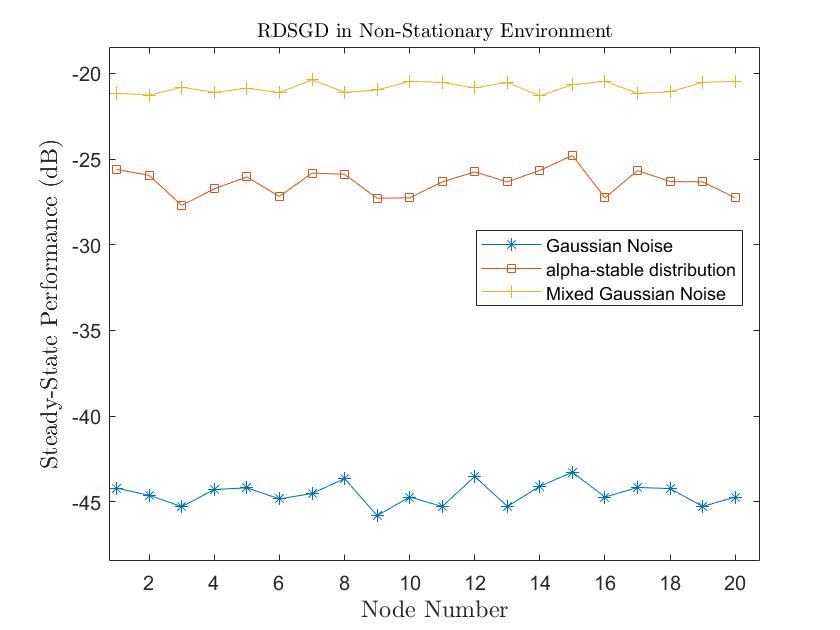
\includegraphics[scale=0.3]{SSP_Noise_non-Stationary.png} 
	\caption{منحنی \lr{MSD} عملکرد گره‌های مختلف در یک شبکه  با 20 گره در حالت پایدار}
	\label{SSP_nonSta}
\end{figure}

\begin{figure}[htbp]  \centering{
		\subfigure[]{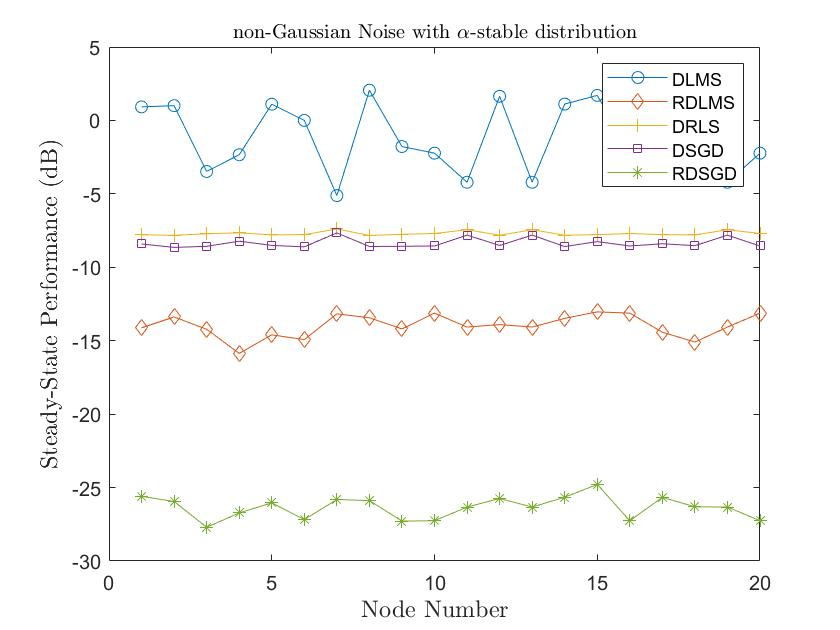
\includegraphics[width=10 cm,height=7 cm]{AlphaStable_SSP.jpg}\label{SSP-alpha}}
		\subfigure[]{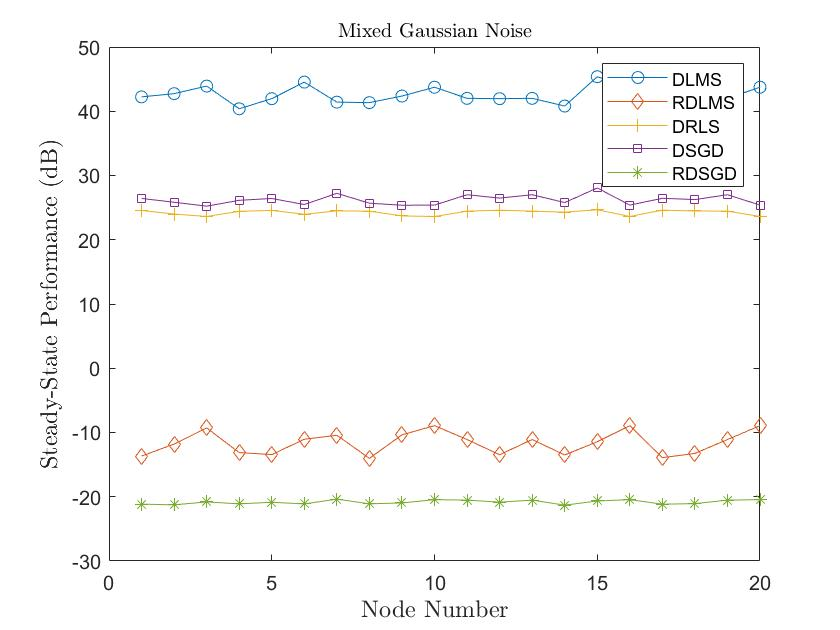
\includegraphics[width=10 cm,height=7 cm]{MixGaussian_SSP.jpg}\label{SSP-mix}}
		\\
		\subfigure[]{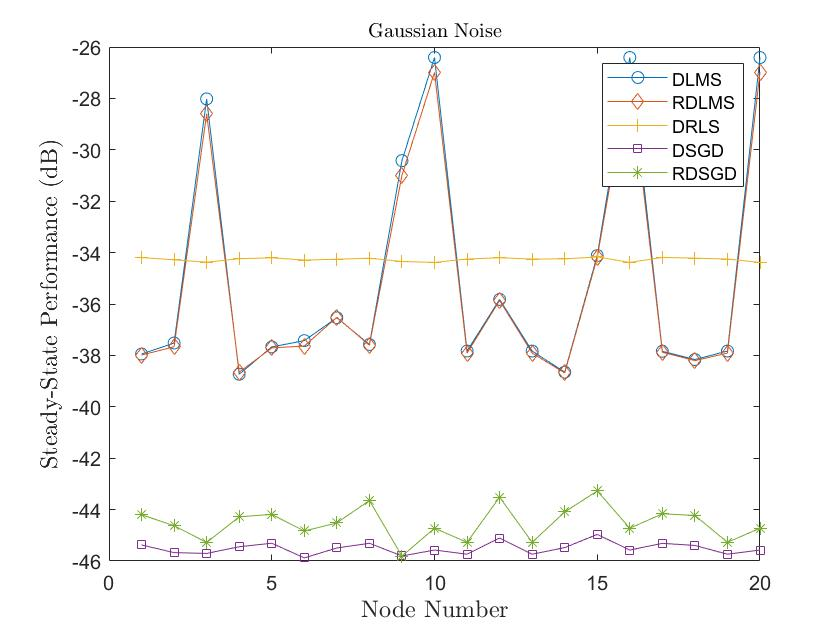
\includegraphics[width=10 cm,height=7 cm]{Gaussian_SSP.jpg}\label{SSP-gaussian}}
	}
	\caption[]{مقایسه رفتار همگرایی  گره‌ها در حالت پایدار  برای تعدادی از الگوریتم‌ها در محیط غیرایستا. الف) نویز الفا پایدار با $SNR=-30 dB$
		ب) نویز گاوسی مخلوط با $SNR=-50 dB$
		ج) نویز گاوسی با $SNR=20 dB$} 
	\label{SSP_non_1}
\end{figure}

\subsection{ارزیابی رویکرد یادگیری توزیع‌شده \lr{FBSP} در مساله شناسایی سیستم}
‌‌‌در این بخش نتایج آزمایشات انجام شده و تحلیل نتایج و مقایسه رویکرد پیشنهادی با دیگر روش‌ها مورد بررسی قرار می‌گیرد. کارایی رویکرد پیشنهادی را در محیطی شبیه‌سازی شده با استفاده از شبیه‌ساز \lr{SimGrid} بررسی می‌کنیم و آن را با روش‌های مشابه \lr{RNA}، \lr{Synch-Switch} و \lr{PSP} مقایسه می‌کنیم. در محیط شبیه‌سازی شده، گره‌ها با پردازنده‌ها و لینک‌هایی با پهنای باند متفاوت تعریف می‌شوند و تعداد یال‌های بین گره‌ها نشان‌دهنده فاصله آنها است که در شبیه‌سازی انجام شده از الگوریتم دیکسترا برای بدست آوردن کوتاه‌ترین مسیر بین هر جفت گره استفاده می‌شود. 

برای رسیدن به یک همگرایی مطلوب، برقراری تعادل بین دفعات اجرای ابرگام سراسری و ابرگام منطقه‌ای بسیار حائز اهمیت است. با هدف کاهش میزان ارتباطات بین گره‌ها و کاهش زمان انتظار آن‌ها، پارامتر کنترلی به نام $qIter$ معرفی شده است که مشخص‌کننده زمان اجرای ابرگام‌ سراسری در رویکرد پیشنهادی \lr{FBSP} است. شروع فرایند یادگیری با ابرگام سراسری بوده و بعد از اجرای $qIter-1$ بار ابرگام منطقه‌ای، یک بار ابرگام سراسری اجرا خواهد شد.

در آزمایش اول همگرایی رویکرد پیشنهادی \lr{FBSP} به ازای مقادیر متفاوت $1$، $10$، $50$ و $100$ برای پارامتر کنترلی $qIter$ بررسی شده است. زمانیکه پارامتر $qIter=1$ است، در واقع تمام ابرگام‌ها به صورت ابرگام سراسری اجرا می‌شوند. همانطور که قبلا هم اشاره شده است، توپولوژی شبکه به صورت یک گراف همبند پیاده‌سازی می‌شود و گره‌های شبکه بر اساس روش خوشه‌بندی ساختار-محتوایی منطقه‌بندی می‌شوند. گراف شبکه از لحاظ تعداد لینک‌ها و ارتباطات هر گره با سایر گره‌ها یا مجموعه همسایگی گره‌ها نباید خلوت باشد. این رویکرد یادگیری توزیع‌شده بر روی گراف‌های خلوت یا گراف‌هایی با تعداد لینک‌های کم به نتایج همگرایی مطلوبی دست پیدا نمی‌کند. شکل \ref{net100} یک شبکه با 100 گره و تعداد لینک‌های مناسب است که آزمایش مورد نظر بر روی این شبکه در یک محیط غیرایستا و آغشته به نویز گاوسی آمیخته اجرا شده است. شکل \ref{qIter1} رفتار همگرایی \lr{FBSP} را در چنین شرایطی به ازای $4$ مقدار متفاوت پارامتر $qIter$ نشان می‌دهد. 

\begin{figure*}[!h]
	\centering
	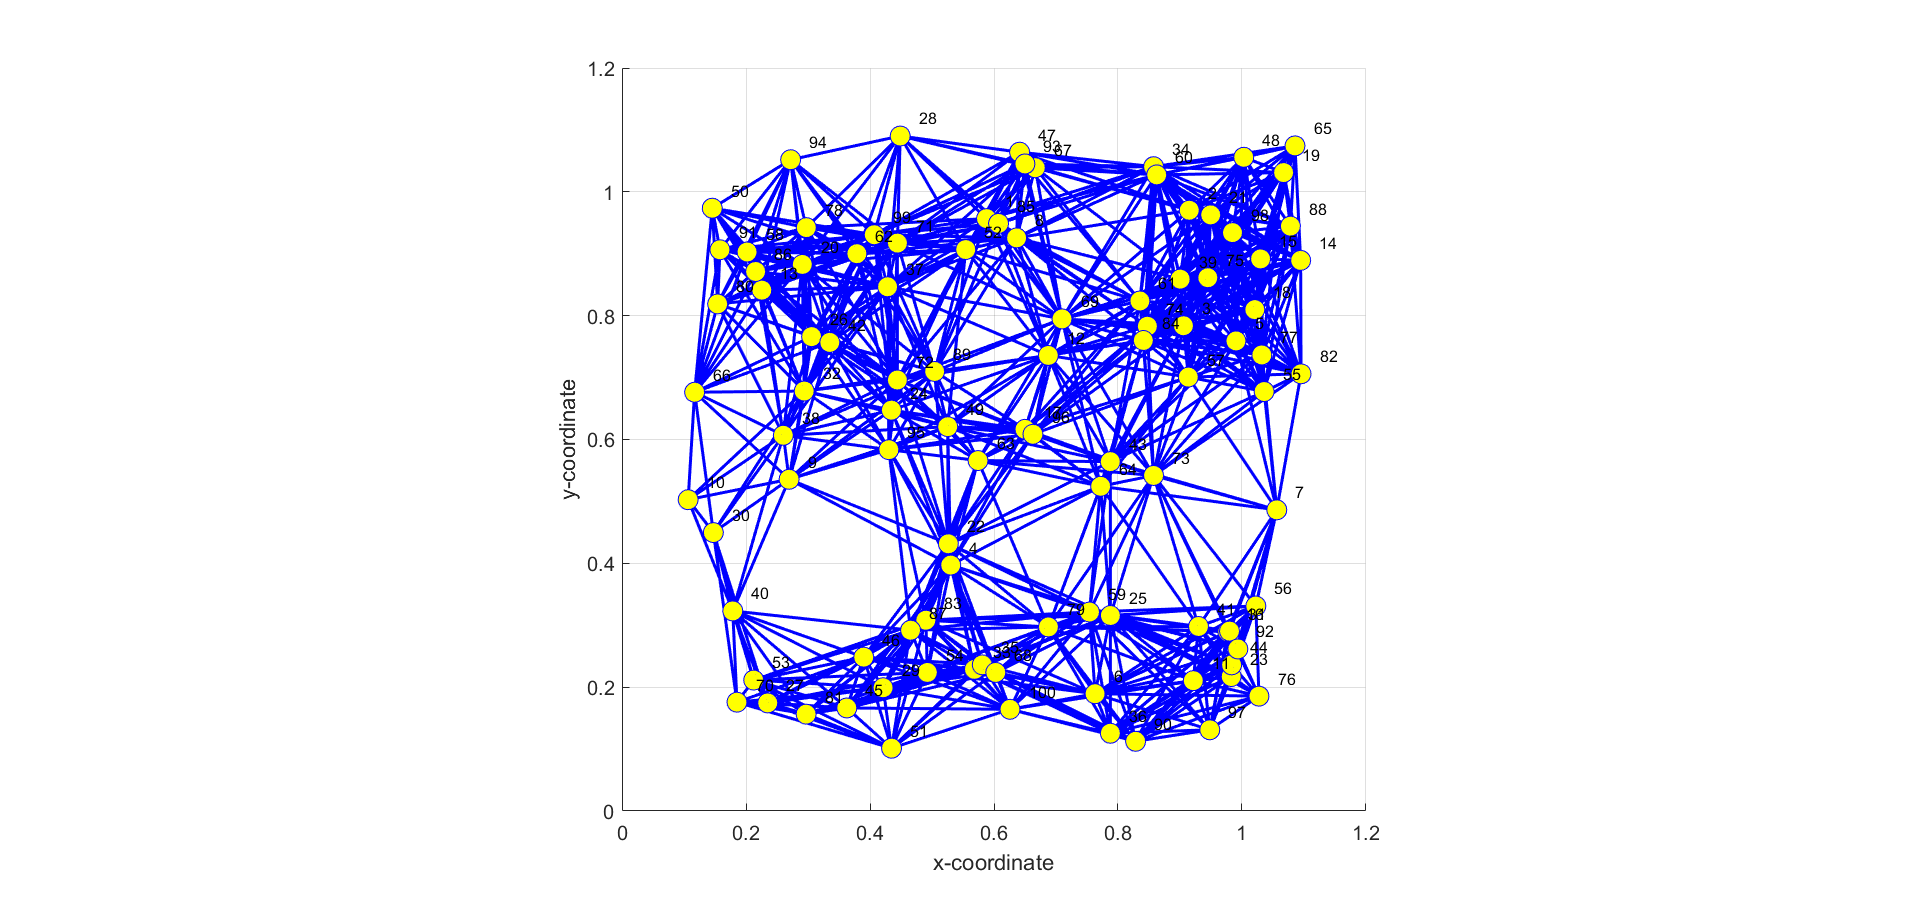
\includegraphics[width=16cm]{Net_100Nodes.png}
	\caption{شبکه‌ای با 100 گره}
	\label{net100}
\end{figure*}



\begin{figure*}[!h]
	\centering
	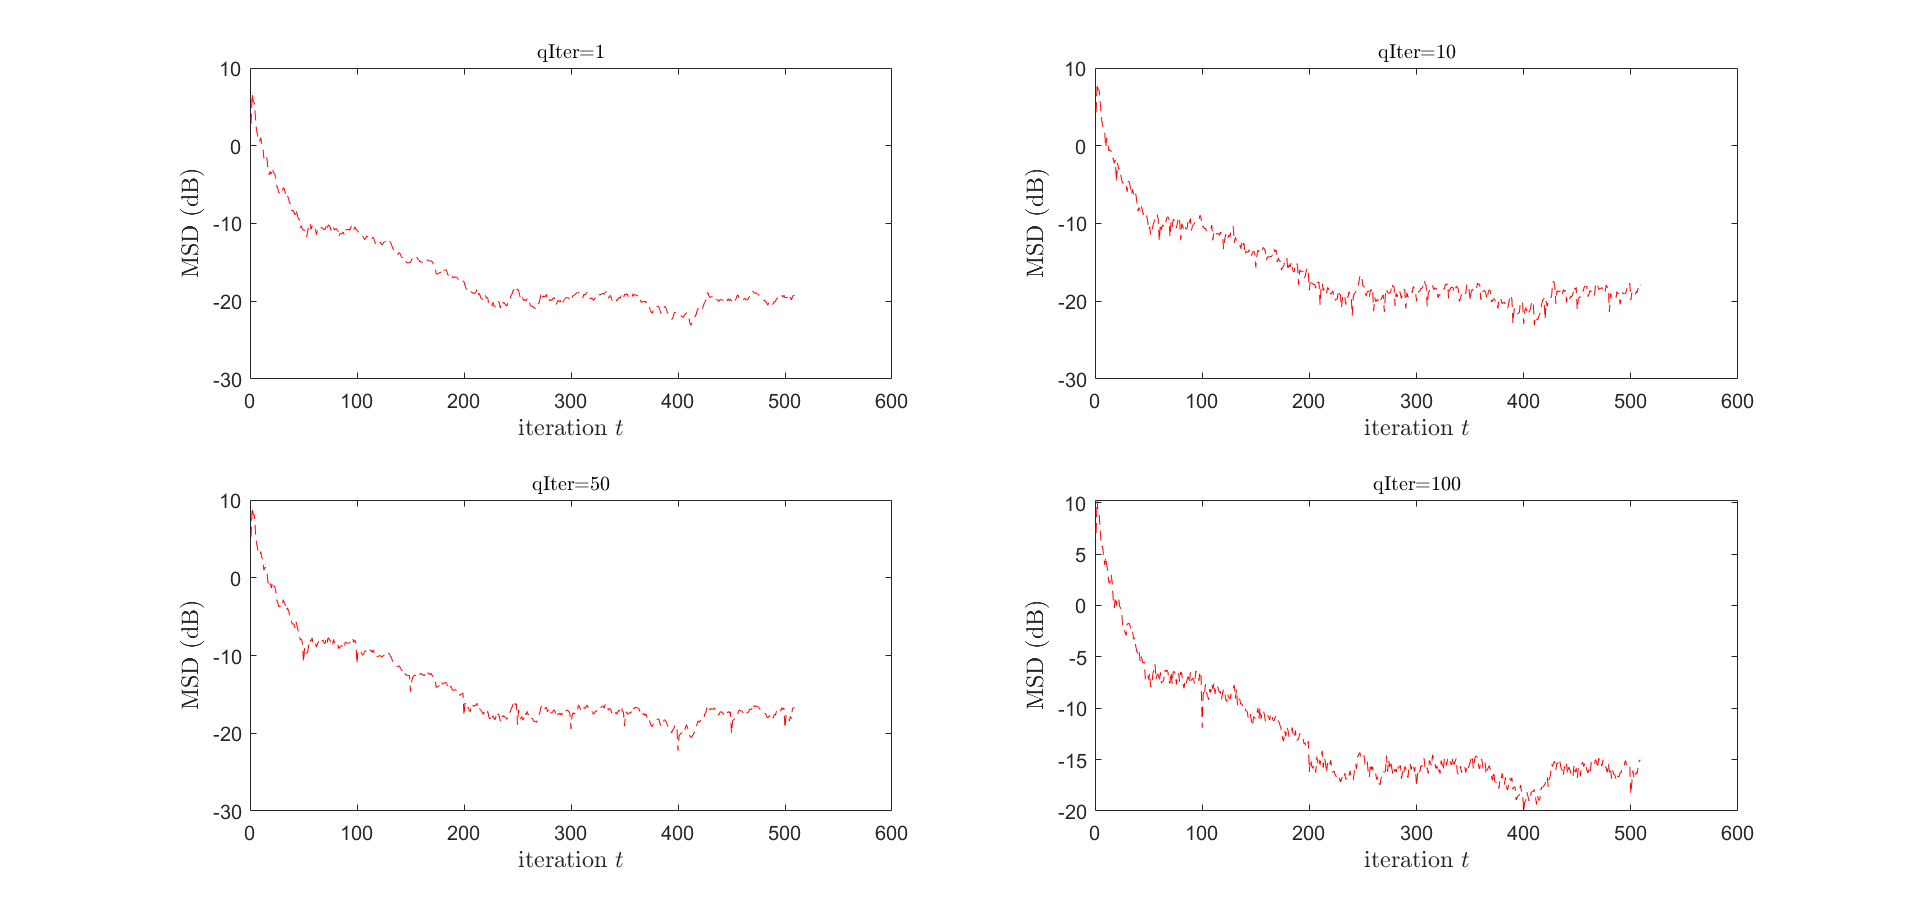
\includegraphics[width=18cm]{FBSP_MixGaussian_500.png}
	\caption{رفتار همگرایی رویکرد پیشنهادی  به ازای مقادیر مختلف پارامتر کنترلی ر یک محیط غیرایستا آغشته به نویز گاوسی آمیخته}
	\label{qIter1}
\end{figure*}
جدول \ref{TableQIter} میانگین زمان انتظار گره‌ها، میانگین مربعات انحراف در حالت پایدار و میانگین تبادلات انجام شده توسط گره‌ها در رویکرد پیشنهادی به ازای مقادیر مختلف پارامتر کنترلی با نماد $qIter$ بر روی $500$ تکرار در یک محیط غیرایستا آغشته به نویز گاوسی آمیخته را نشان می‌دهد. همان طور که دیده می‌شود، اجرای ابرگام‌های منطقه‌ای باعت می‌شود در حالت پایدار رویکرد پیشنهادی به میانگین خطای بالاتری همگرا ‌شود اما قادر است تاثیر بسیار مطلوبی بر کاهش زمان انتظار گره‌ها داشته باشد. به طور میانگین این رویکرد به ترتیب منجر به کاهش $34/67\%$، $63.1\%$ و $70.57\%$ زمان انتظار گره‌ها به ازای مقادیر $qIter=10$، $qIter=50$ و $qIter=100$ می‌شود. همچنین این رویکرد قادر است سبب کاهش $27.83\%$ و $36.73\%$ و $50.37\%$ در تعداد ارتباطات به ترتیب به ازای مقادیر $qIter=10$، $qIter=50$ و $qIter=100$ شود.
\begin{table}
	\centering
	\caption{رفتار رویکرد پیشنهادی به ازای مقادیر مختلف پارامتر کنترلی }\label{TqIter}
	\begin{tabular}{|c|c|c|c|}\hline
		\lr{Avg. Num. of Comm. per iter.}&\lr{Avg. Idle Time(s)} & \lr{MSD(dB)}& \lr{Approach}  \\\hline
		$20.23$ & $30$ & $-19.27$  & \lr{FBSP with qIter=1}\\\hline
		$14.6$ &  $19.6$ & $-17.93$& \lr{FBSP with qIter=10}\\\hline
		$11.8$ & $11.07$  & $-16.69$&\lr{FBSP with qIter=50}\\\hline
		$10.04$ & $8.83$  & $-15.03$ & \lr{FBSP with qIter=100}\\\hline
	\end{tabular}
	\label{TableQIter}
\end{table}
با افزایش مقدار پارامتر کنترلی $qIter$ تعداد دفعات اجرای ابرگام سراسری در طول اجرای فرآیند یادگیری توزیع‌شده و به دنبال آن ارتباطات و تبادلات سراسری گره‌ها کمتر خواهد شد. دریافت اطلاعات توسط یک گره از کلیه گره‌های همسایه (ارتباطات سراسری) در مرحله ترکیب یادگیری توزیع‌شده انتشاری به همگرایی سریع‌تر به خطای کمتر در حالت پایدار کمک می‌کند. اما با این آزمایش  بررسی شد که اگر برقراری ارتباطات سراسری توسط هر گره به یک بار به ازای $qIter$ بار برقراری ارتباطات منطقه‌ای  کاهش یابد، نتایج قابل قبولی بر اساس معیارهای میانگین زمان انتظار گره‌ها، انحراف میانگین مربعات در حالت پایدار و میانگین تبادلات انجام شده حاصل خواهد شد (جدول \ref{TableQIter} را ببینید). همان طور که در شکل \ref{qIter1} نشان داده شده است، در طی فرآیند یادگیری توزیع‌شده در تکرارهایی که ابرگام سراسری اجرا می‌شود پیک‌هایی در منحنی \lr{MSD} دیده می‌شود و بعد از چند تکرار منحنی بر اساس نتایج بدست آمده از تبادلات سراسری روند قبلی خود را با تمایل به خطا کمتر ادامه خواهد داد. این آزمایش برای محیط‌ غیرایستا آغشته به نویز گاوسی و محیط غیرایستا آغشته به نویز آلفا-پایدار نیز تکرار شد و منحنی \lr{MSD} آن‌ها به ترتیب در شکل‌های \ref{qIter2} و \ref{qIter3} نشان داده شده است. 

\begin{figure*}[!h]
	\centering
	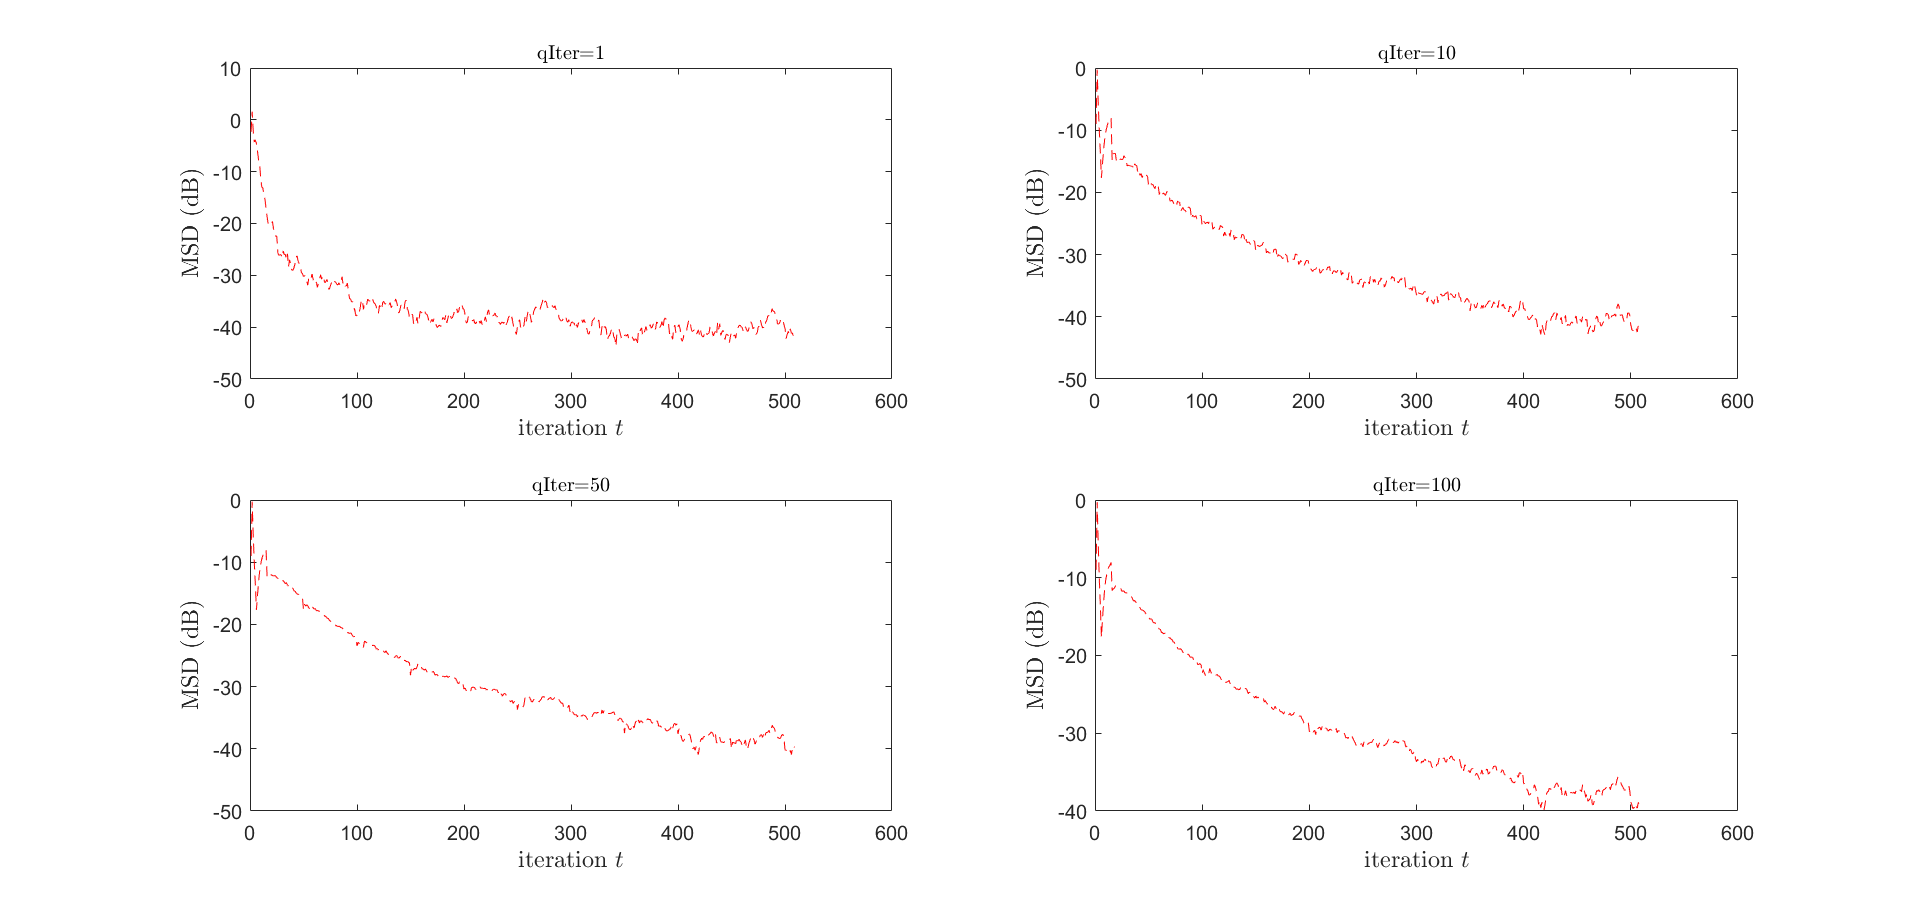
\includegraphics[width=18cm]{FBSP_Gaussian_500_.png}
	\caption{رفتار همگرایی رویکرد پیشنهادی  به ازای مقادیر مختلف پارامتر کنترلی در یک محیط غیرایستا آغشته به نویز گاوسی}
	\label{qIter2}
\end{figure*}

\begin{figure*}[!h]
	\centering
	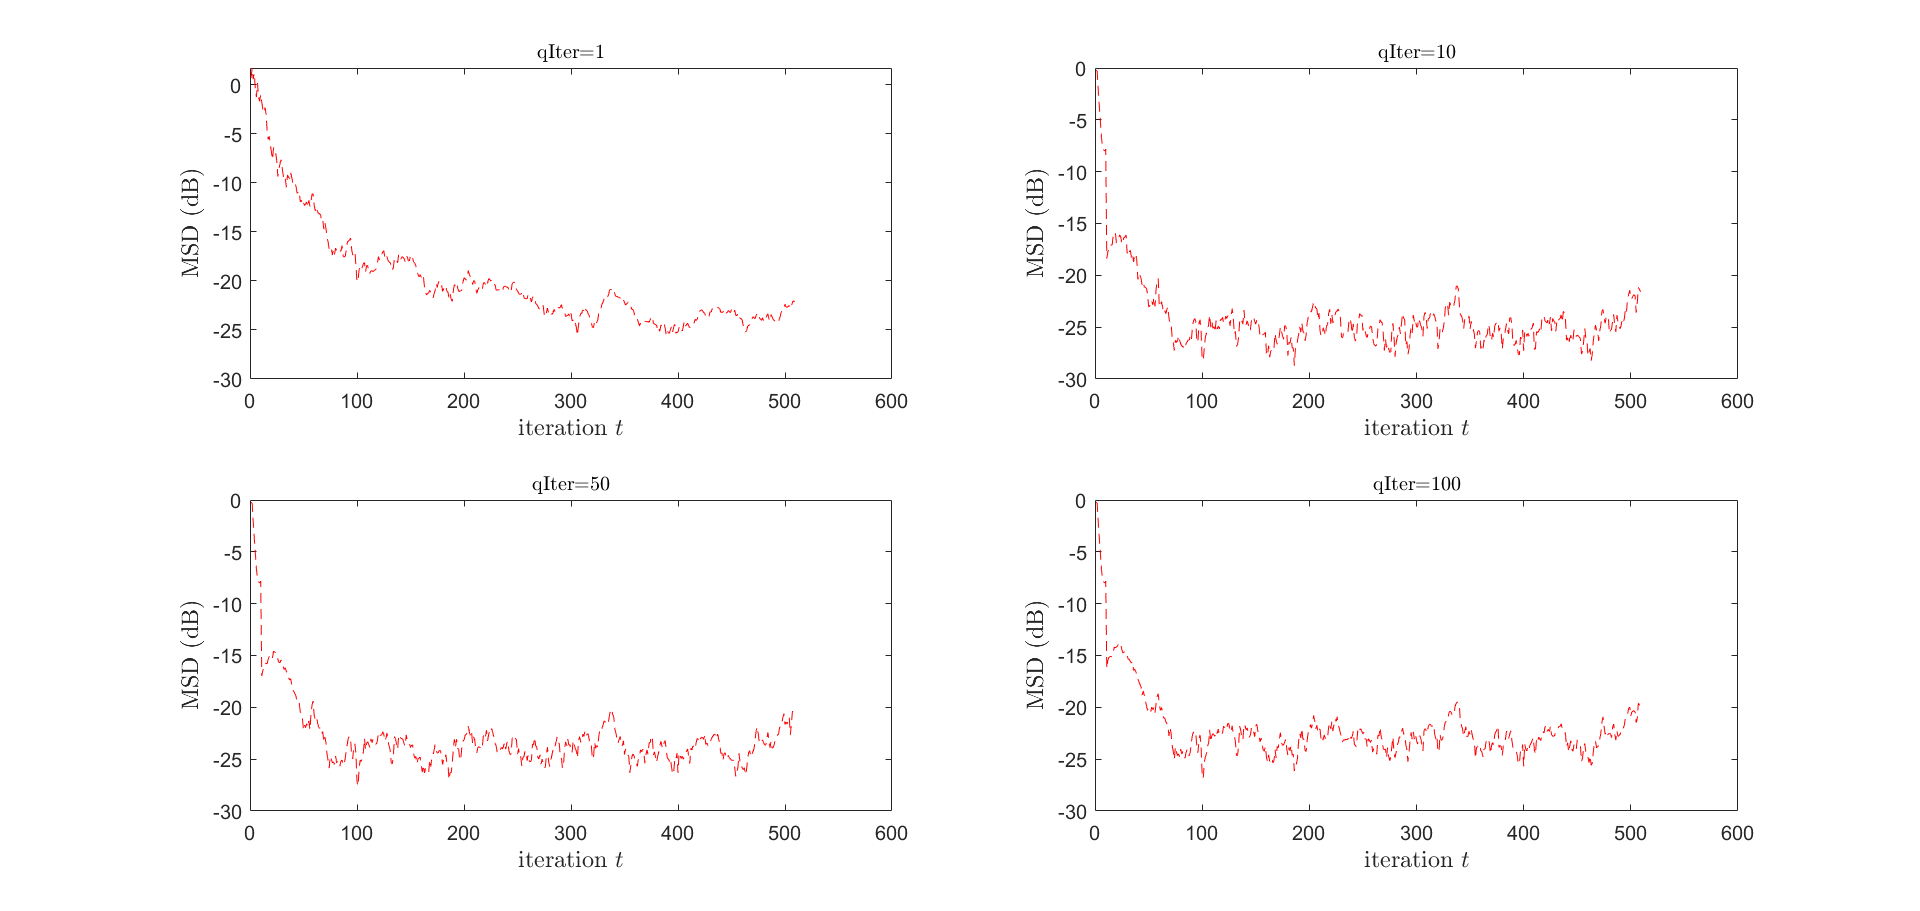
\includegraphics[width=18cm]{FBSP_Alpha_500.png}
	\caption{رفتار همگرایی رویکرد پیشنهادی  به ازای مقادیر مختلف پارامتر کنترلی در یک محیط غیرایستا آغشته به نویز آلفا-پایدار}
	\label{qIter3}
\end{figure*}

در آزمایش دوم میانگین زمان انتظار گره‌ها و انحراف میانگین مربعات در رویکرد پیشنهادی در دو حالت $qIter=1$ و $qIter=50$ با سه رویکرد یادگیری توزیع‌شده \lr{RNA}، \lr{Synch-Switch} و \lr{PSP} در سه محیط غیرایستا آغشته به نویز گاوسی آمیخته، گاوسی و آلفا-پایدار مقایسه شده است. نتایج مقایسه رویکرد پیشنهادی \lr{FBSP} با سه رویکرد دیگر از حیث میانگین زمان انتظار گره‌ها در زمان همگام‌سازی در شکل \ref{Idle1} نشان داده شده است. همان طور که دیده می‌شود، زمان انتظار گره‌ها در رویکرد \lr{FBSP} با پارامتر کنترلی $qIter=1$ (در این حالت \lr{FBSP} تقریبا مشابه \lr{BSP} رفتار می‌کند) از کلیه رویکردهای مورد مقایسه بیشتر است. این اختلاف زیاد به این دلیل است که تمام همگام‌سازی‌ها در \lr{FBSP} با پارامتر $qIter=1$ به صورت همگام‌سازی سراسری اجرا می‌شوند. رویکرد \lr{RNA} در هر ابرگام زمان اتمام کار تنها یک گره نماینده تصادفی را ملاک زمان اجرای همگام‌سازی قرار می‌دهد و به همین دلیل میانگین زمان انتظار گره‌ها در این رویکرد کمتر از سایر رویکردهای مورد مقایسه است. در این آزمایش \lr{FBSP} با پارامتر $qIter=50$ از لحاظ زمان انتظار تقریبا مشابه رویکرد \lr{PSP} عمل می‌کند. در رویکرد \lr{PSP} زمان همگام‌سازی گره‌ها بر اساس زمان اتمام کار محاسباتی حداقل $20$ درصد از گره‌ها تعیین می‌گردد که این گره‌ها به صورت تصادفی انتخاب می‌شوند.

\begin{figure*}[!h]
	\centering
	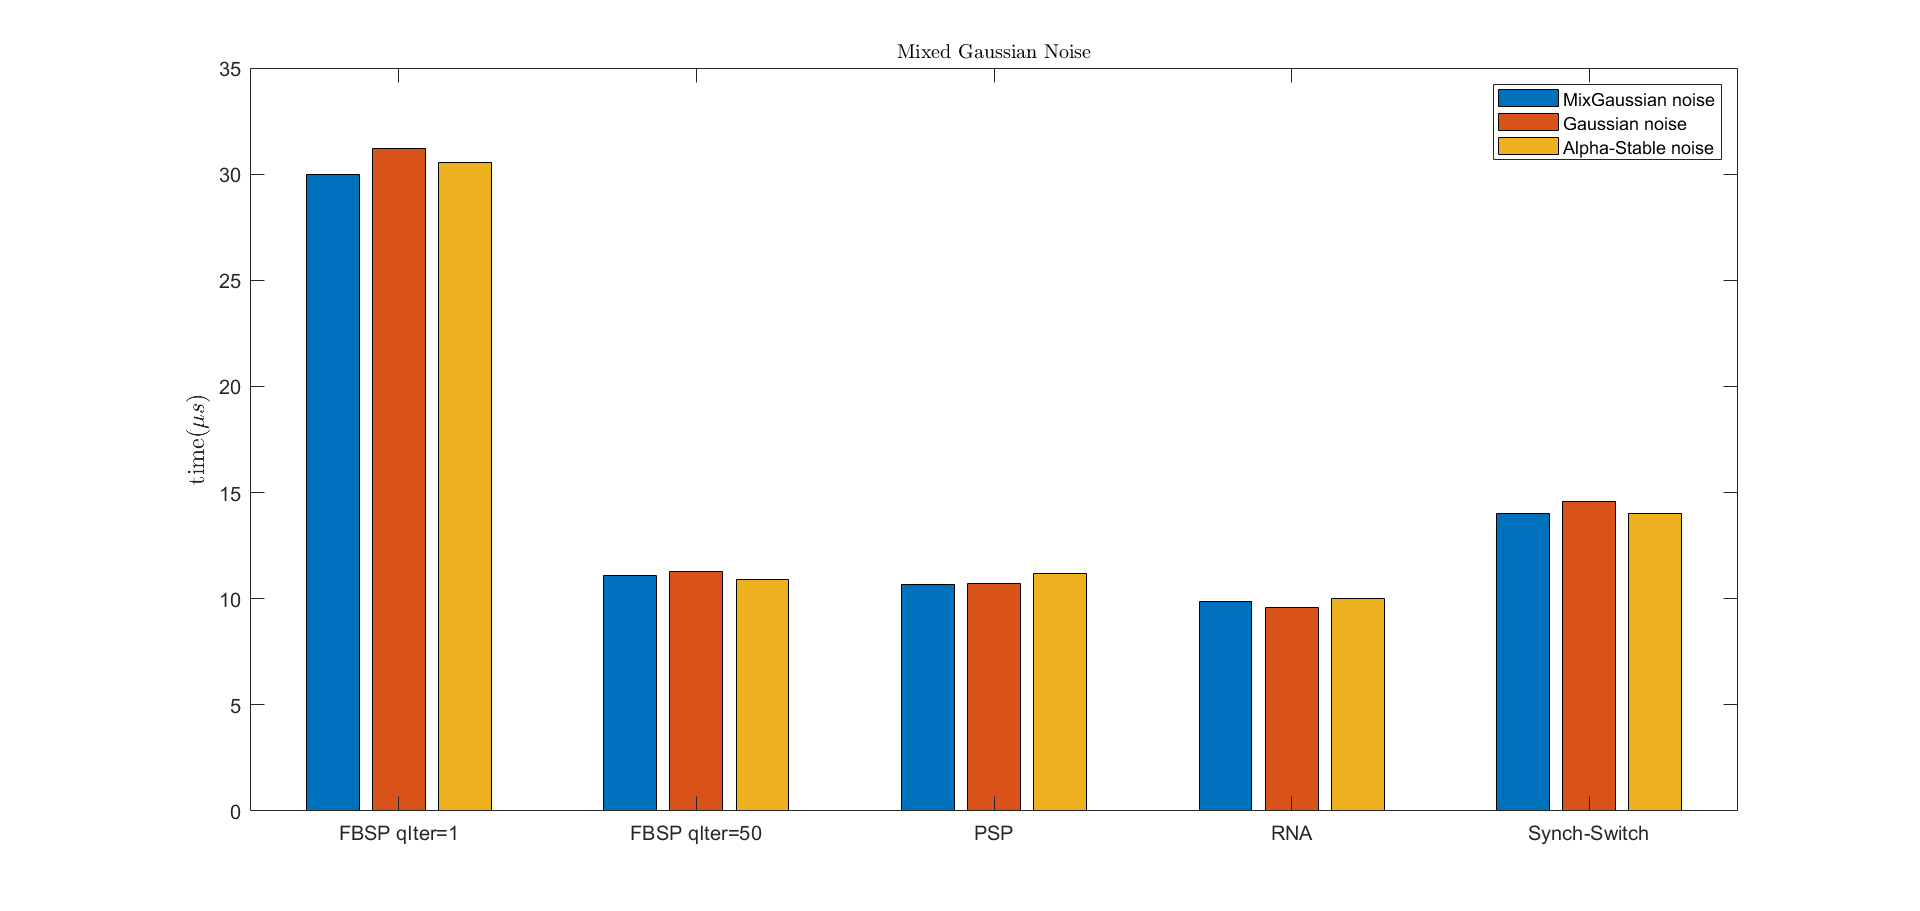
\includegraphics[width=18cm]{IdleTime_All.png}
	\caption{مقایسه زمان انتظار گره‌ها در رویکرد پیشنهادی با سایر رویکردهای یادگیری توزیع‌شده مشابه}
	\label{Idle1}
\end{figure*}
همچنین در شکل \ref{Idle2} انحراف میانگین مربعات در حالت پایدار رویکرد پیشنهادی با رویکردهای یادگیری توزیع‌شده مشابه در سه محیط غیرایستا آغشته به نویز گاوسی آمیخته، گاوسی و آلفا-پایدار مقایسه شده است. شکل \ref{Idle2} نشان می‌دهد که رویکرد \lr{FBSP} با پارامتر $qIter=1$ قادر است در حضور هر سه نوع نویز محیطی به خطا کمتری نسبت به سایر رویکردها همگرا می‌شود. رویکرد \lr{FBSP} با پارامتر کنترلی $qIter=50$ در موقعیت دوم نسبت به سایر رویکردهای مورد مقایسه قرار دارد که البته با توجه به نتایج ارائه شده در شکل \ref{Idle1} و با در نظر گرفتن توانایی رویکرد \lr{FBSP} با پارامتر کنترلی $qIter=50$ در کاهش زمان انتظار گره‌ها در طی فرآیند یادگیری، می‌توان ادعا کرد که نتایج انحراف میانگین مربعات در حالت پایدار قابل قبول می‌باشند. در نتیجه اختلاف کمی که بین  نتایج \lr{MSD} حالت پایدار رویکرد پیشنهادی در حالت  $qIter=50$ و $qIter=1$ دیده می‌شود، قابل چشم‌پوشی است. رویکرد \lr{RNA} به دلیل استناد به اتمام کار تنها یک گره تصادفی در هر ابرگام و به احتمال زیاد تبادل و استفاده از داده‌های کهنه و ناهماهنگی توسط گره‌های شبکه به مقادیر خطا بیشتری در حالت پایدار همگرا می‌شود. جدول \ref{AllTableFBSP} به طور خلاصه نتایج مقایسه رویکرد پیشنهادی با سایر رویکردهای مشابه را در محیط غیرایستا و در حضور نویز گاوسی آمیخته، نویز گاوسی و نویز آلفا-پایدار نشان می‌دهد. 

\begin{figure*}[!ht]
	\centering
	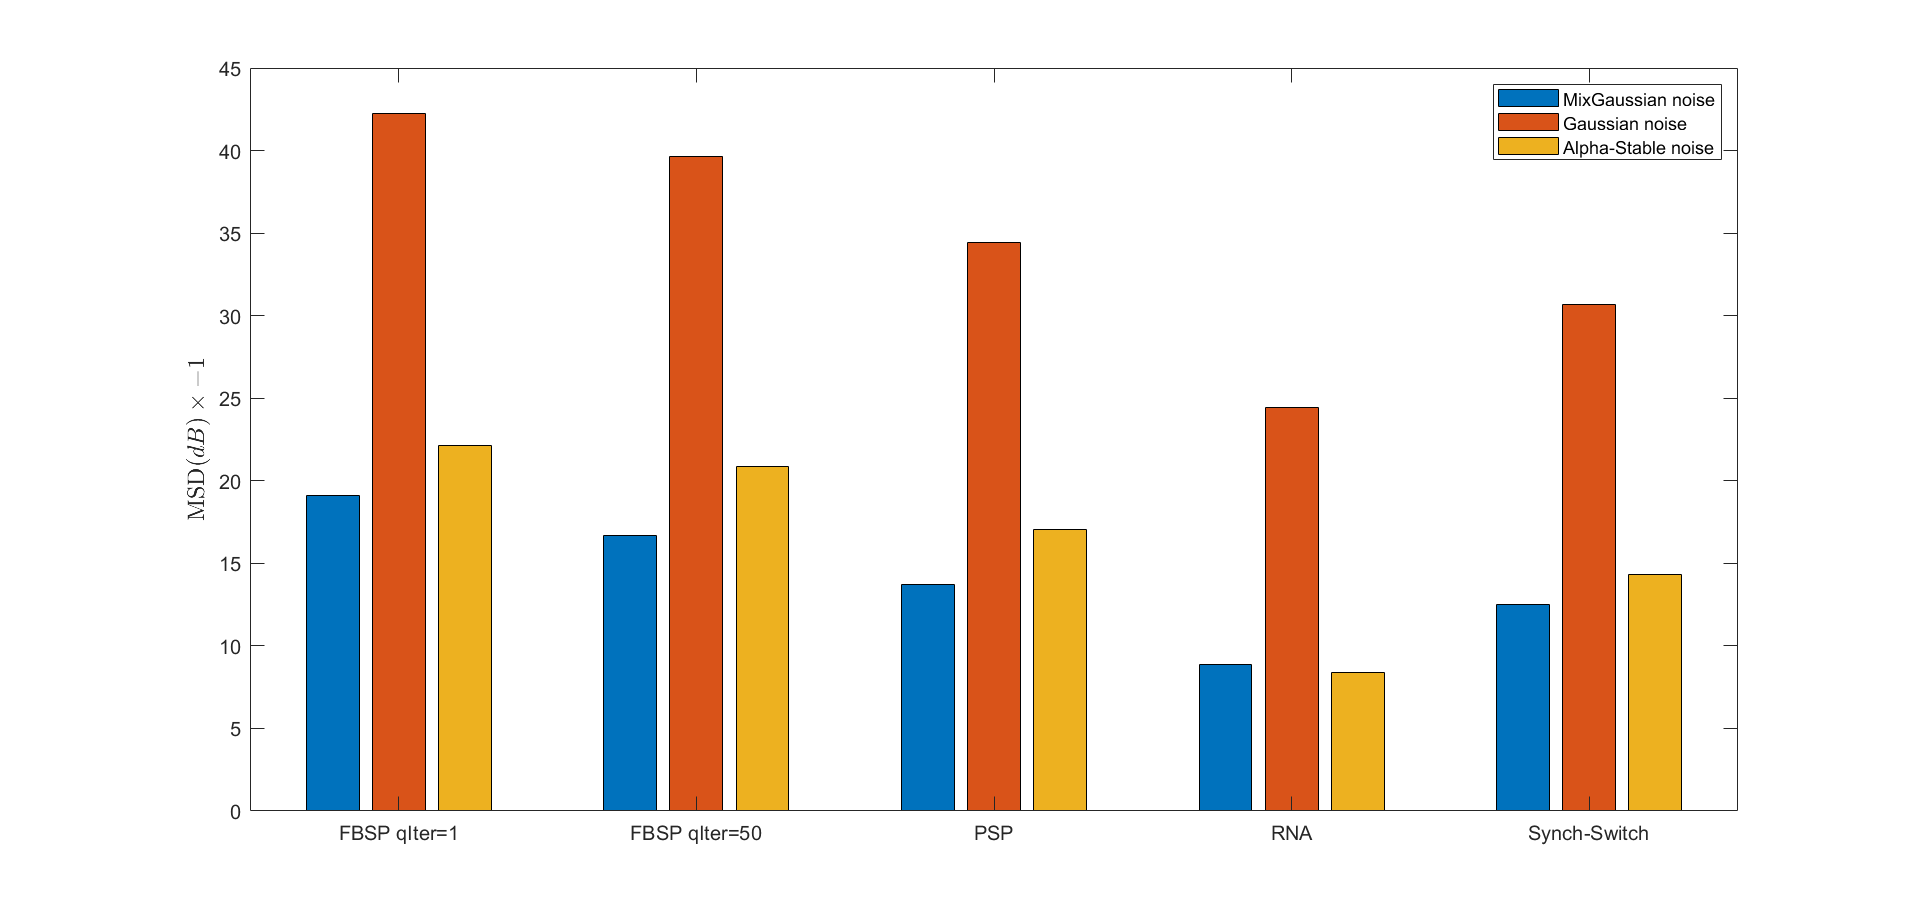
\includegraphics[width=18cm]{MSD_All.png}
	\caption{مقایسه انحراف میانگین مربعات رویکرد پیشنهادی با سایر رویکردهای یادگیری توزیع‌شده مشابه}
	\label{Idle2}
\end{figure*}

\begin{table}[!ht]
	\centering
	\caption{مقایسه رفتار رویکرد پیشنهادی با سایر رویکردهای مشابه}
	\begin{tabular}{|c|c|c|c|c|c|l|}
		\hline
		\multicolumn{2}{|c|}{\lr{Alpha-Stable}} & \multicolumn{2}{|c|}{\lr{Gaussian}} & \multicolumn{2}{|c|}{\lr{MixGaussian}} & \multirow{2}{*}{\lr{Approach}}\\
		\lr{Idle Time(s)} & \lr{MSD(dB)} & \lr{Idle Time(s)} & \lr{MSD(dB)} &\lr{Idle Time(s)} & \lr{MSD(dB)} & \\
		\hline
		$30.53$ & $-22.12$ & $31.2$ & $-42.25$ & $30$ & $-19.27$ & \lr{FBSP with qIter=1}\\\hline
		$10.89$ & $-20.86$ & $11.3$ & $-39.66$ & $11.07$  & $-16.69$&\lr{FBSP with qIter=50}\\\hline
		$10$ & $-8.4$ & $9.60$ & $-24.44$ & $9.883$  & $-8.86$ & \lr{RNA}\\\hline
		$14$ & $-14.3$ & $14.6$ & $-30.68$ & $14.03$  & $-12.5$ & \lr{Synch-Switch}\\\hline
		$11.2$ & $-17.06$ & $10.72$ & $-34.45$ & $10.65$  & $-13.71$ & \lr{PSP}\\\hline
	\end{tabular}
	\label{AllTableFBSP}
\end{table}

در آزمایشی دیگر مقاومت رویکرد پیشنهادی در برابر محیط‌های ناهمگن با سایر رویکردها مورد بررسی و مقایسه قرار گرفته است. در این آزمایش میزان کندی گره‌های شبکه در آزمایش قبلی به $2$ برابر $2\times$ و $10$ برابر $10\times$ تغییر داده می‌شود تا مقاومت رویکردهای یادگیری توزیع‌شده در برابر محیط‌های ناهمگن مختلف ارزیابی گردد. شکل \ref{Robust_Heterogeneous} رفتار همگرایی رویکرد \lr{FBSP} با پارامتر کنترلی $qIter=50$ در $500$ تکرار را در محیط‌های مختلف ناهمگن در مقایسه با سه رویکرد \lr{RNA}، \lr{PSP} و \lr{Synch-Switch} در یک محیط غیرایستا آغشته به نویز گاوسی آمیخته نشان می‌دهد. 

\begin{figure*}[!ht]
	\centering
	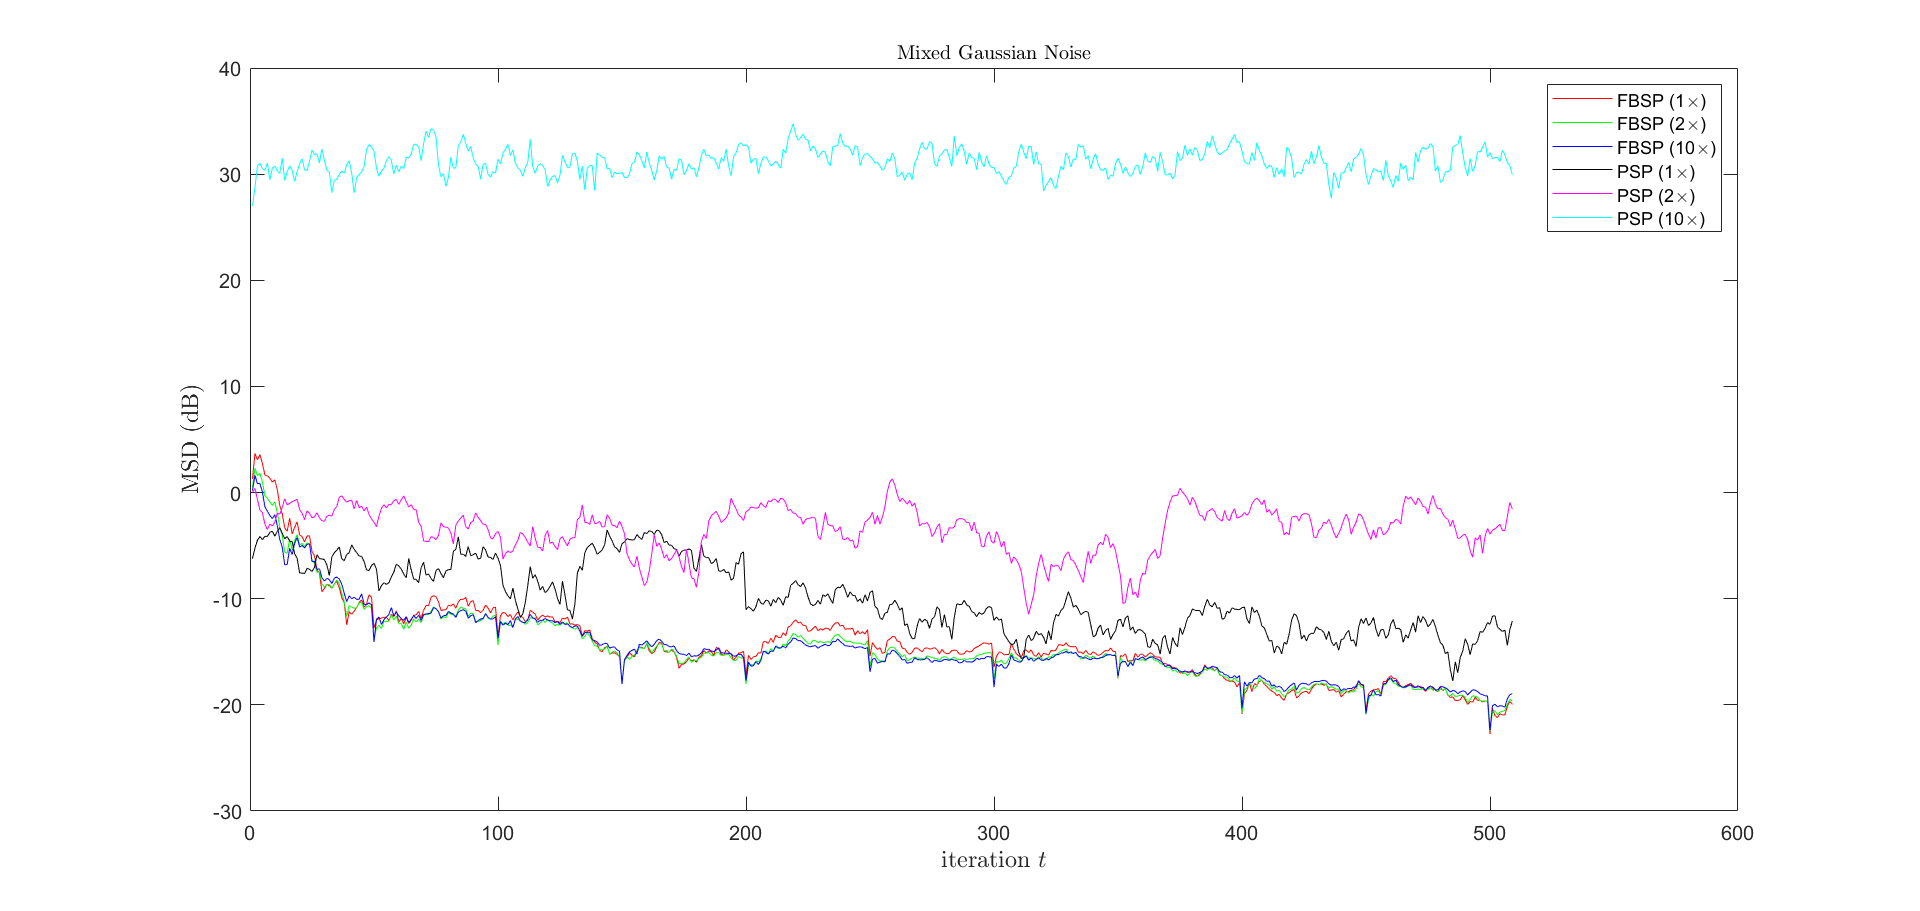
\includegraphics[width=17cm]{Heterogenous.png}
	\caption{مقاومت رویکرد یادگیری توزیع‌شده در محیط‌های ناهمگن مختلف}
	\label{Robust_Heterogeneous}
\end{figure*}

همان طور که مشاهده می‌شود، رویکرد پیشنهادی \lr{FBSP} در برابر درجه ناهمگنی‌های مختلف محیط اجرایی مقاوم است و رفتار همگرایی آن در حالت‌های $1X$، $2X$ و $10X$ تقریبا یکسان می‌باشد. در این آزمایش مقاومت رویکرد یادگیری توزیع‌شده \lr{PSP} که نسبت به دو رویکرد مورد مقایسه دیگر نتایج بهتر و نزدیک‌تری به \lr{FBSP} ارائه می‌دهد، مورد بررسی قرار گرفت. نتایج ارائه شده در \ref{Robust_Heterogeneous} دلالت بر عدم مقاومت رویکرد \lr{PSP} در برابر محیط‌های اجرایی با درجه ناهمگنی مختلف دارند. در نتیجه رویکرد پیشنهادی \lr{FBSP} علاوه بر توانایی در کاهش زمان انتظار گره‌ها و کاهش تعداد ارتباطات، در برابر محیط‌های اجرایی  با درجه ناهمگنی مختلف نیز مقاوم است. 

\subsection{ارزیابی رویکرد یادگیری توزیع‌شده \lr{FBSP} در مساله پیش‌‌بینی بازار بورس}
در سال‌های اخیر، پیش‌بینی بازار سهام موضوع بسیار مهمی برای محققان بوده و مطالعات متعددی برای پیش‌بینی حرکت بازار سهام با استفاده از الگوریتم‌های مختلف یادگیری ماشین انجام شده است. بازار سهام با نوسانات شدید، غیرخطی بودن و تغییرات زیاد متغیرهای محیطی توصیف می‌شود. دلایل مختلفی پشت نوسانات، خطی نبودن بازار سهام وجود دارد، از جمله گرانی سهام شرکت، گزارش زیان شرکت، جنگ تجاری، رکود بازار جهانی، تنش‌های ژئوپلیتیکی و بیماری‌های همه‌گیر مانند ویروس کرونا را می‌توان ذکر کرد.

در این بخش یک مجموعه از داده‌های بورس ایران شامل اطلاعات 736 شرکت مورد استفاده قرار گرفته است. در این مجموعه داده، اطلاعات هر شرکت به صورت یک ساختار داده به شرح زیر در دسترس می‌باشد:
\begin{itemize}
	\item \lr{Name}: نام كامل شرکت
	\item \lr{Namad}: نام مختصر یا معروف شرکت
	\item \lr{Data}: برداری از اطلاعات مختلف مربوط به شرکت 
	\item  \lr{HDate}: تاریخ روزهایی که اطلاعات مربوط به آنها در بردار \lr{Data} وجود دارد
	\item \lr{HPrice}: ساختار داده‌ای که شامل اطلاعات مختلف مربوط به قیمت شرکت موردنظر در هر كدام از
	روزها در \lr{HDate}
	\begin{itemize}
		\item \lr{High}: بالاترین قیمت هر سهم در هر روز
		\item  \lr{Low}: کمترین قیمت سهم در هر روز
		\item \lr{Close}: میانگین وزن‌دار قیمت معامله‌های انجام شده در نیم ساعت پایانی روز
		\item \lr{Last}: قیمت اخرین معامله ی انجام شده
		\item \lr{First}: قیمت اولین معامله ی انجام شده
		\item \lr{Open}: میانگین وزن‌دار قیمت معامله‌های انجام شده در نیم ساعت اغازین روز
		\item \lr{ValTrades}: ارزش معاملات
		\item \lr{NumShares}: تعداد سهام
		\item \lr{NumTrades}: تعداد معاملات
		\item \lr{Grad}: گرادیان
		\item \lr{FHigh}: فلیپ شده \lr{High}
		\item \lr{Flow}: فلیپ شده \lr{Low}
		\item \lr{FClose}: فلیپ شده \lr{Close} و غیره
	\end{itemize}
	\item \lr{FHDate}: فلیپ شده \lr{HDate}
	\item \lr{Len}: اطلاعات زمانی مرتبط با داده (تعداد روزهای هفته، ماه و سال و ...)
	\item \lr{RL}: اطلاعات مربوط به حقیقی و حقوقی‌ها	
\end{itemize}



رویکرد \lr{FBSP} با کمک الگوریتم‌های یادگیری توزیع‌شده تطبیقی می‌توانند رفتار غیرخطی در سیگنال‌های بورس را تشخیص داده و به نتایج پیش‌بینی بسیار دقیقی منجر شوند. در این بخش، از الگوریتم \lr{RDSGD} برای پیش‌بینی روز-آینده\footnote{\lr{next-day}} روند سهام استفاده شده است و قابلیت پیش‌بینی رویکرد پیشنهادی بر اساس الگوریتم‌‌های یادگیری توزیع‌شده \lr{RDSGD}، \lr{DLMS}، \lr{DRLS}، \lr{DSGD}، \lr{SGD} و \lr{RDLMS} مورد ارزیابی قرار گرفته است. برای این منظور از مجموعه داده‌های مربوط به معاملات شرکت‌های مختلف در بازار سهام ایران استفاده شده است. آزمایش‌‌ها بر روی یکی از سیگنال‌های ارائه شده در این مجموعه داده به نام \lr{Fclose} انجام می‌شود. این سیگنال میانگین وزن‌دار ارزش تراکنش‌های انجام شده در نیم ساعت آخر روز را نشان می‌دهد. به عنوان نمونه در شکل \ref{Compaies} سیگنال \lr{fclose} شرکت‌های داروسازی کاسپین تامین \lr{Caspian}، شرکت سرمایه‌گذاری ملت \lr{VMelat}، شرکت کشت و صنعت شریف‌آباد \lr{ZSharif} و شرکت پرمیت \lr{Permit} نشان داده شده است.

\begin{figure}[htbp]  \centering{
		\subfigure[]{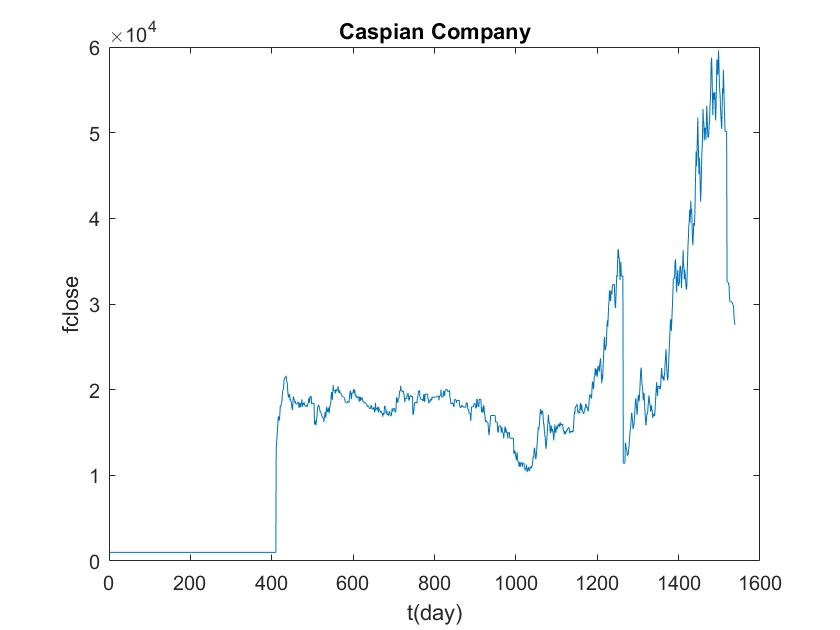
\includegraphics[width=8 cm,height=5 cm]{Caspian.jpg}\label{fig:Caspian}}
		\subfigure[]{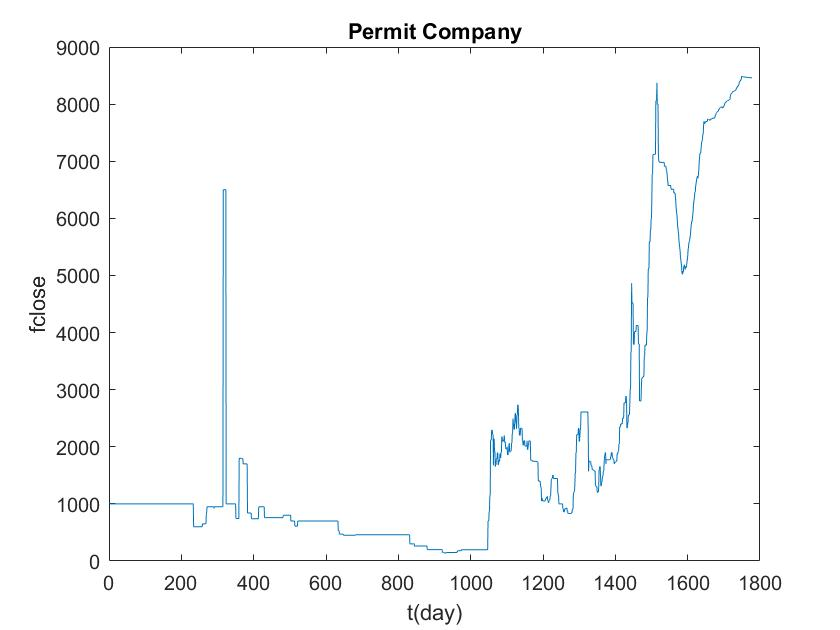
\includegraphics[width=8 cm,height=5 cm]{Permit.jpg}\label{fig:BuAli}}
		\\
		\subfigure[]{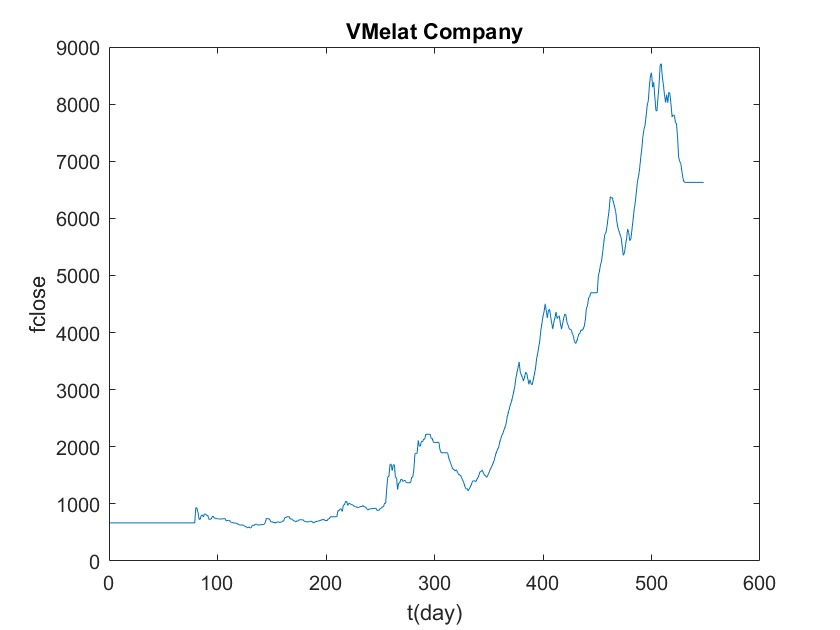
\includegraphics[width=8 cm,height=5 cm]{VMelat_fclose.png}\label{fig:Khazar}}
		\subfigure[]{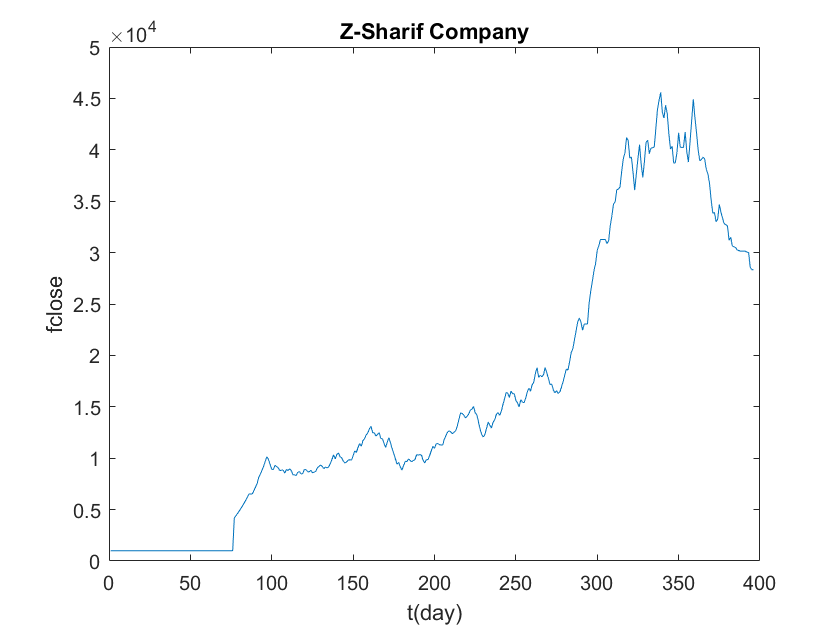
\includegraphics[width=8 cm,height=5 cm]{ZSharif_fclose.png}\label{fig:Permit}}
	}
	\caption[]{سیگنال \lr{Fclose} برخی از شرکت‌ها. الف) \lr{Caspian company}
		ب) \lr{Permit Company}
		ج) \lr{VMelat Company}
		د) \lr{ZSharif Company}
	}
	\label{Compaies}
\end{figure}

هدف از این آزمایش بررسی توانایی الگوریتم‌های یادگیری توزیع‌شده مختلف رویکرد \lr{FBSP} در مساله پیش‌بینی است. با توجه به اینکه ارائه و نمایش منحنی‌های پیش‌بینی شرکت‌های متعدد مجموعه داده موردنظر خارج از حوصله این نوشته است، در این آزمایش تنها به نمایش منحنی پیش‌بینی چند شرکت (ذکر شده در \ref{Compaies}) در ازای شش الگوریتم یادگیری توزیع‌شده اکتفا خواهد شد. در شکل‌های \ref{PredictCompare1} تا \ref{PredictCompare4} توانایی رویکرد پیشنهادی در پیش‌بینی سیگنال \lr{Fclose} شرکت‌های  \lr{Caspian}، \lr{Permit}، \lr{VMelat} و \lr{ZSharif} نشان داده شده است. همان‌طور که دیده می‌شود، الگوریتم‌های \lr{LMS} هم نسخه انتشاری آن (\lr{DLMS}) و هم نسخه انتشاری مقاوم آن (\lr{RDLMS}) قادر به پیش‌بینی سیگنال‌های بازار سهام نمی‌باشند. همچنین، الگوریتم \lr{SGD} شبیه الگوریتم \lr{RDLMS} عمل می‌کند و قادر به پیش‌بینی این سیگنال‌ها نمی‌باشد. الگوریتم \lr{RDSGD}، \lr{DSGD} , \lr{DRLS} در پیش‌بینی سیگنال‌ها موفق‌تر بوده و قادر به پیش‌بینی سیگنال \lr{Fclose} شرکت‌ها با خطای کمتری در مقایسه با الگوریتم‌های دسته \lr{LMS} هستند. \lr{DSGD} در مقایسه با \lr{RDSGD} پیش‌بینی‌ها را با دقت بالاتری ارائه می‌دهد و از این لحاظ مشابه \lr{DRLS} عمل می‌کند.

\begin{figure*}[!h]
	\centering
	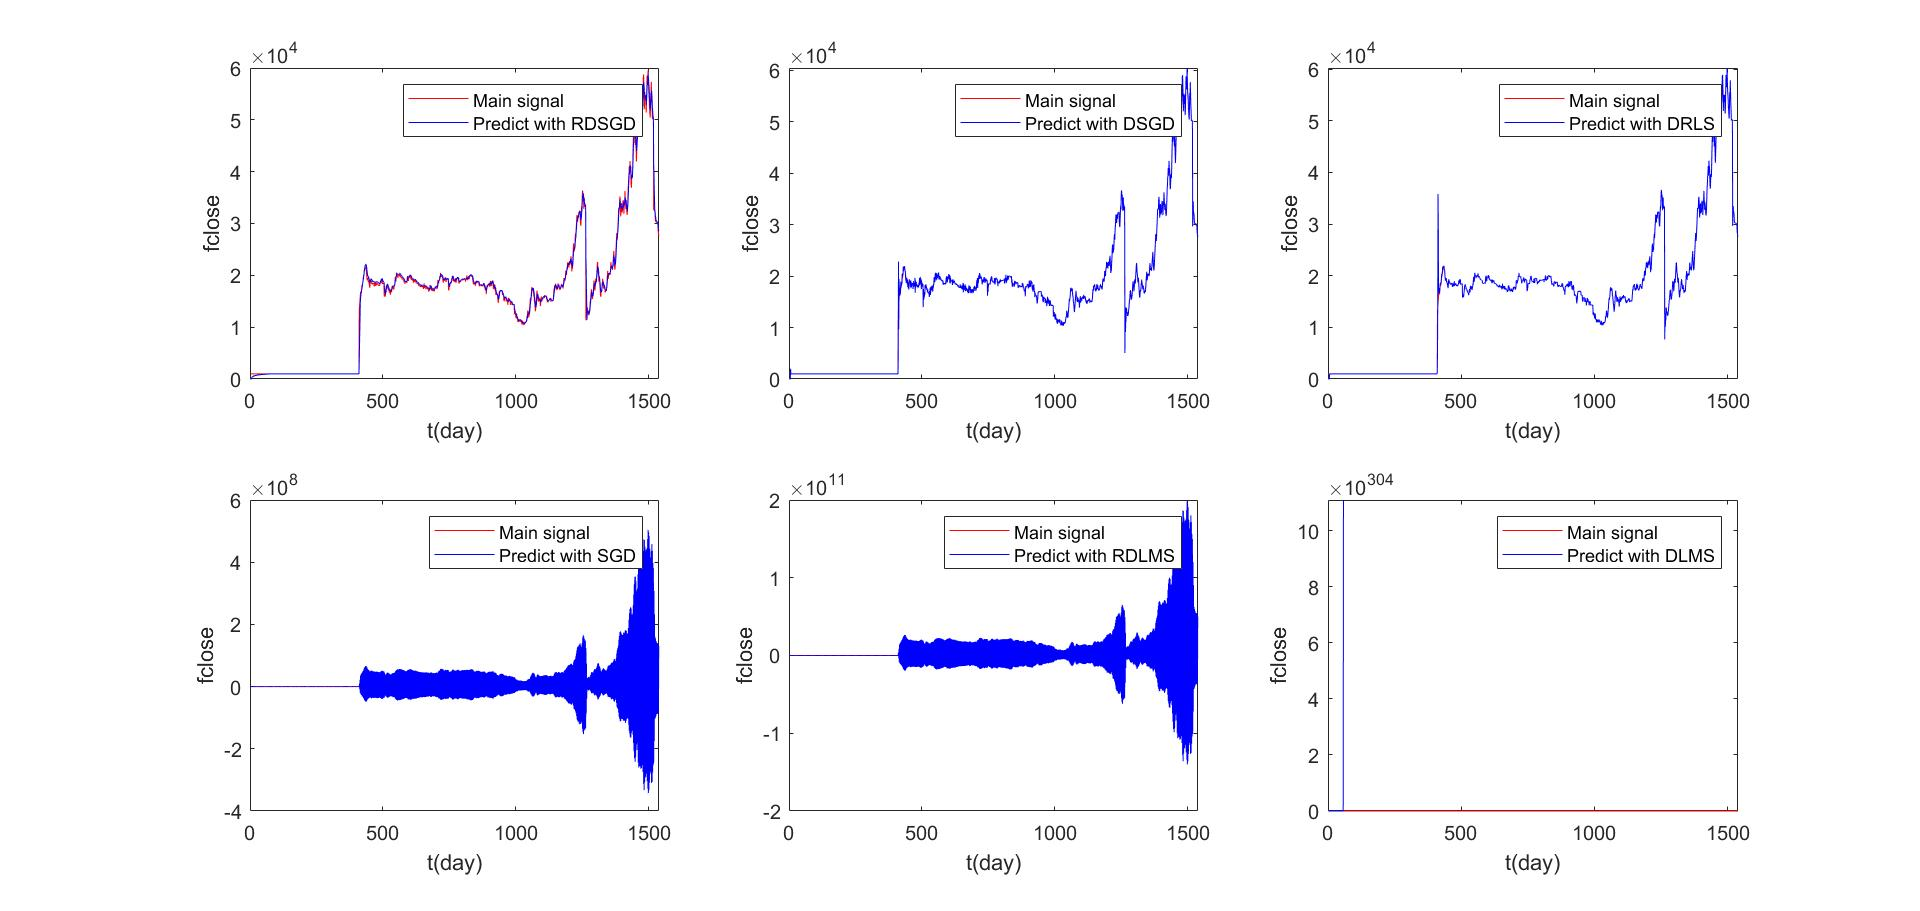
\includegraphics[width=16cm]{CompareFigs_6_Caspian.jpg}
	\caption{مقایسه الگوریتم‌های یادگیری توزیع‌شده رویکرد \lr{FBSP} در پیش‌بینی سیگنال بازار سهام شرکت داروسازی کاسپین تامین}
	\label{PredictCompare1}
\end{figure*}

\begin{figure*}[!h]
	\centering
	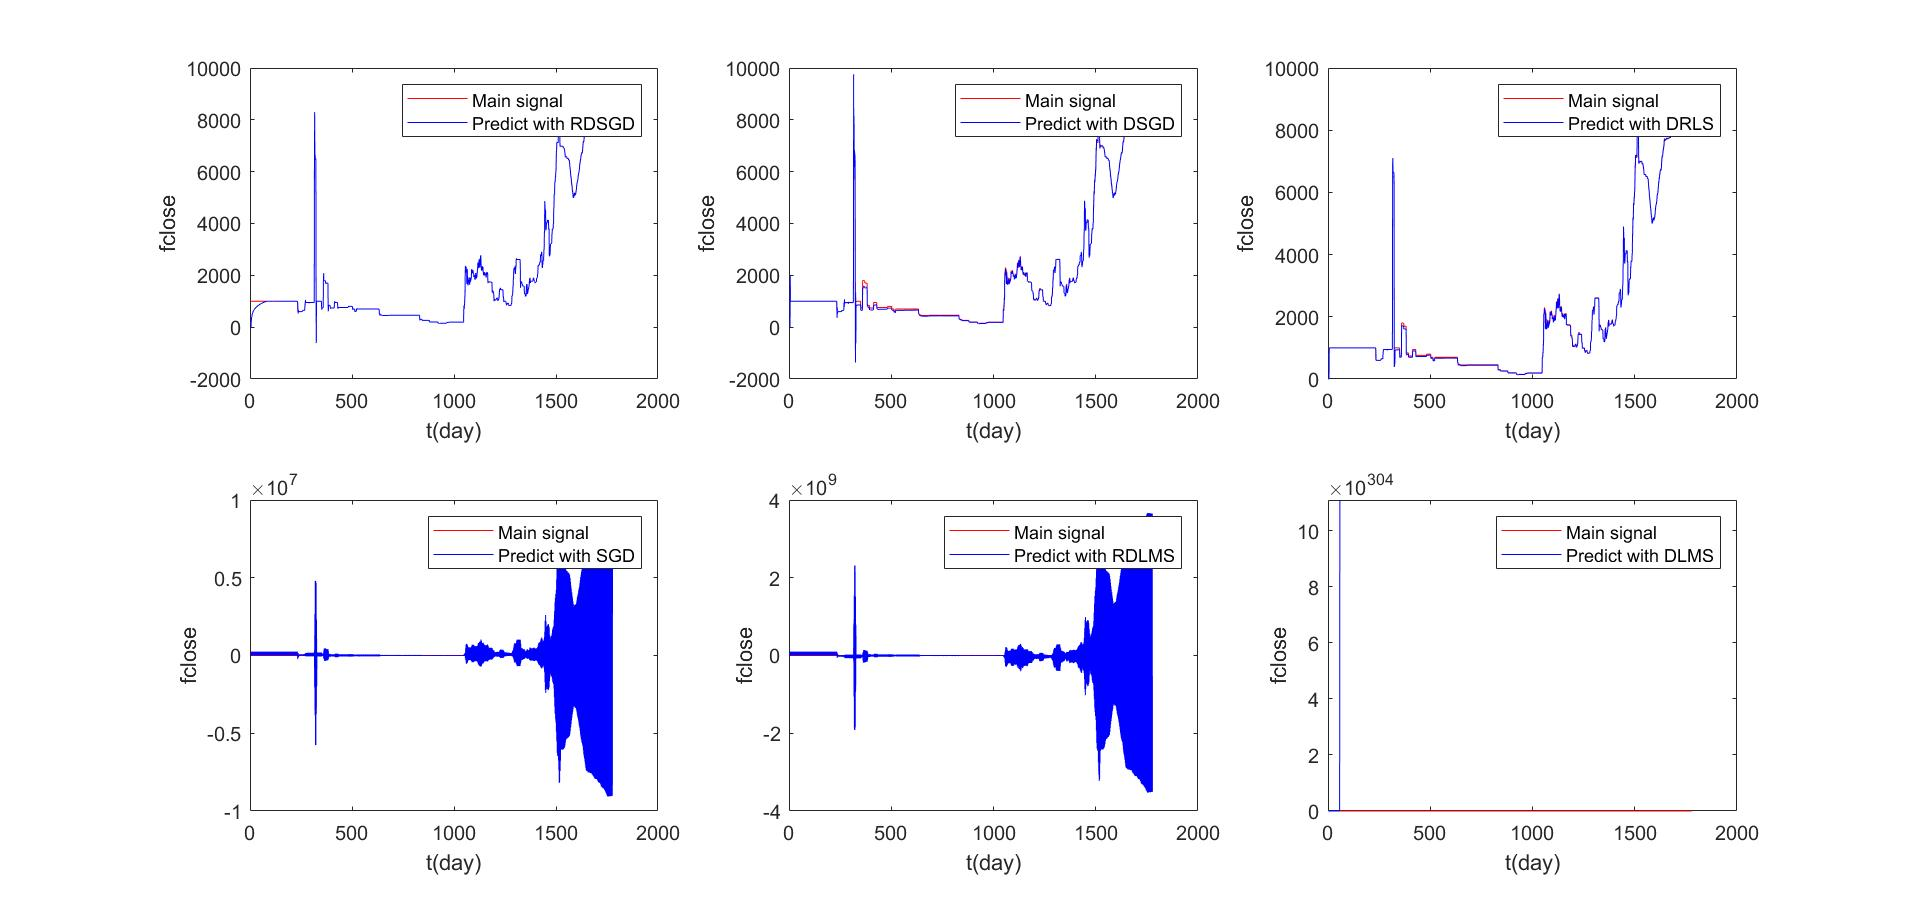
\includegraphics[width=16cm]{CompareFigs_6_Permit.jpg}
	\caption{مقایسه الگوریتم‌های یادگیری توزیع‌شده رویکرد \lr{FBSP} در پیش‌بینی سیگنال بازار سهام شرکت پرمیت}
	\label{PredictCompare2}
\end{figure*}

\begin{figure*}[!h]
	\centering
	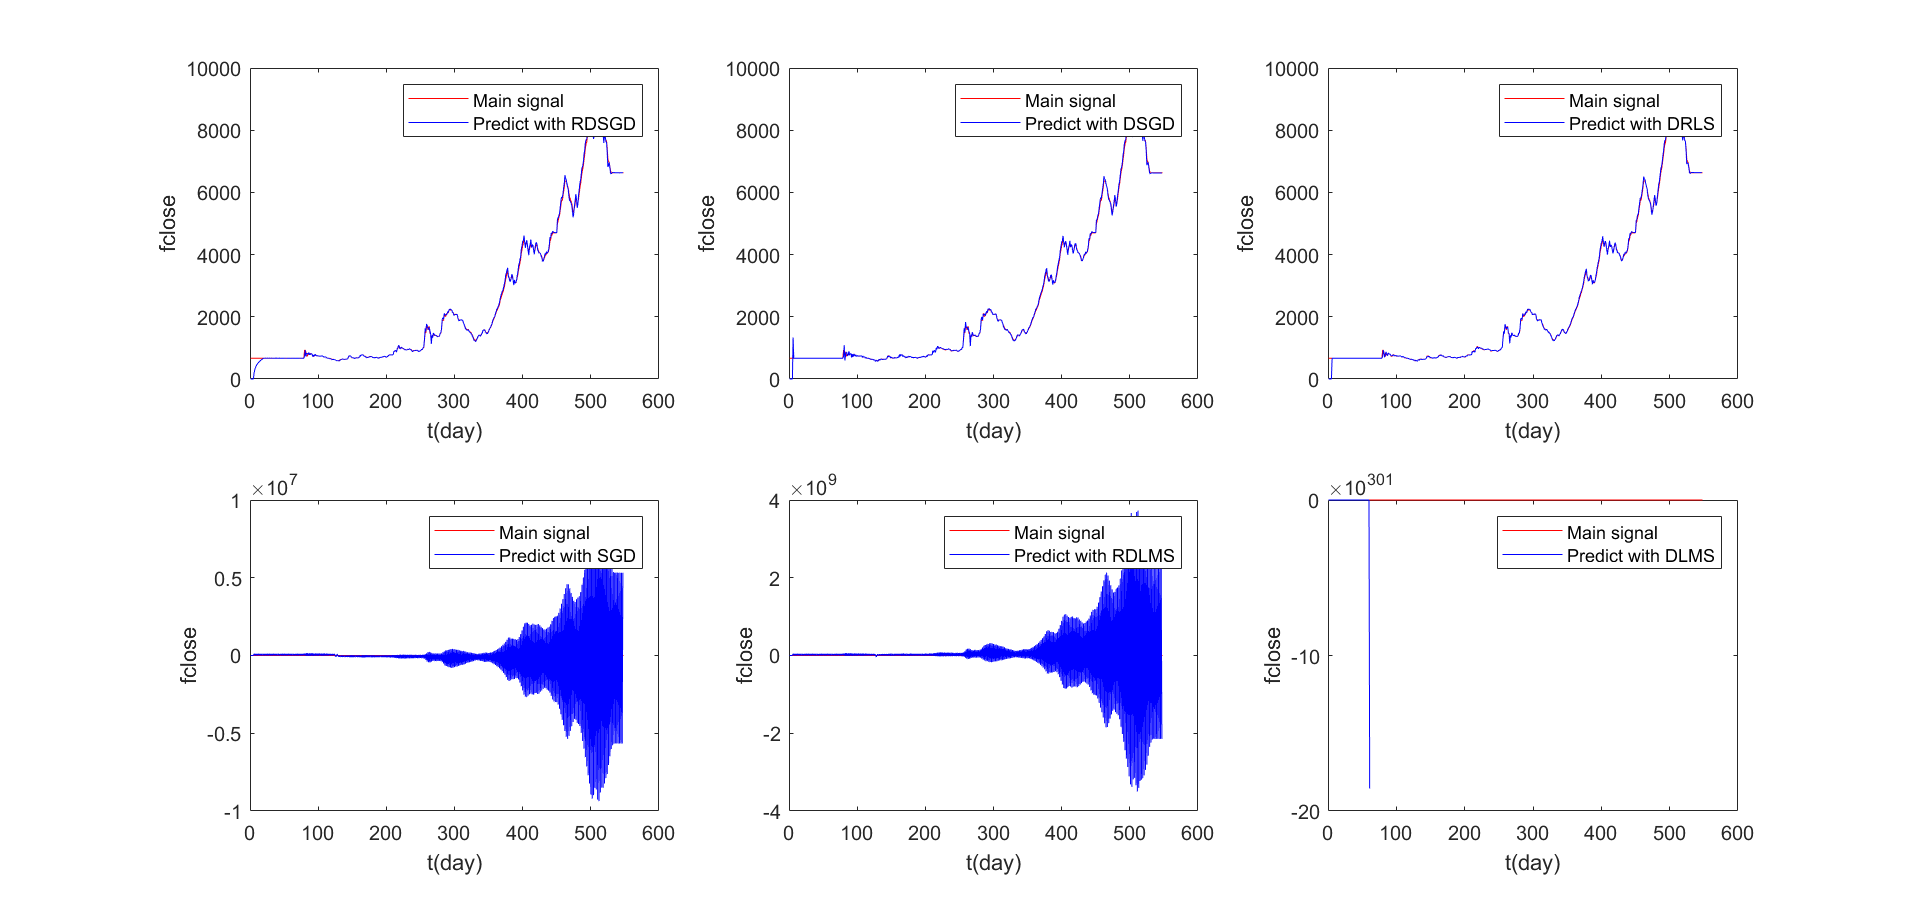
\includegraphics[width=16cm]{VMelat_Pre.png}
	\caption{مقایسه الگوریتم‌های یادگیری توزیع‌شده رویکرد \lr{FBSP} در پیش‌بینی سیگنال بازار سهام شرکت سرمایه گذاری ملت }
	\label{PredictCompare3}
\end{figure*}

\begin{figure*}[!h]
	\centering
	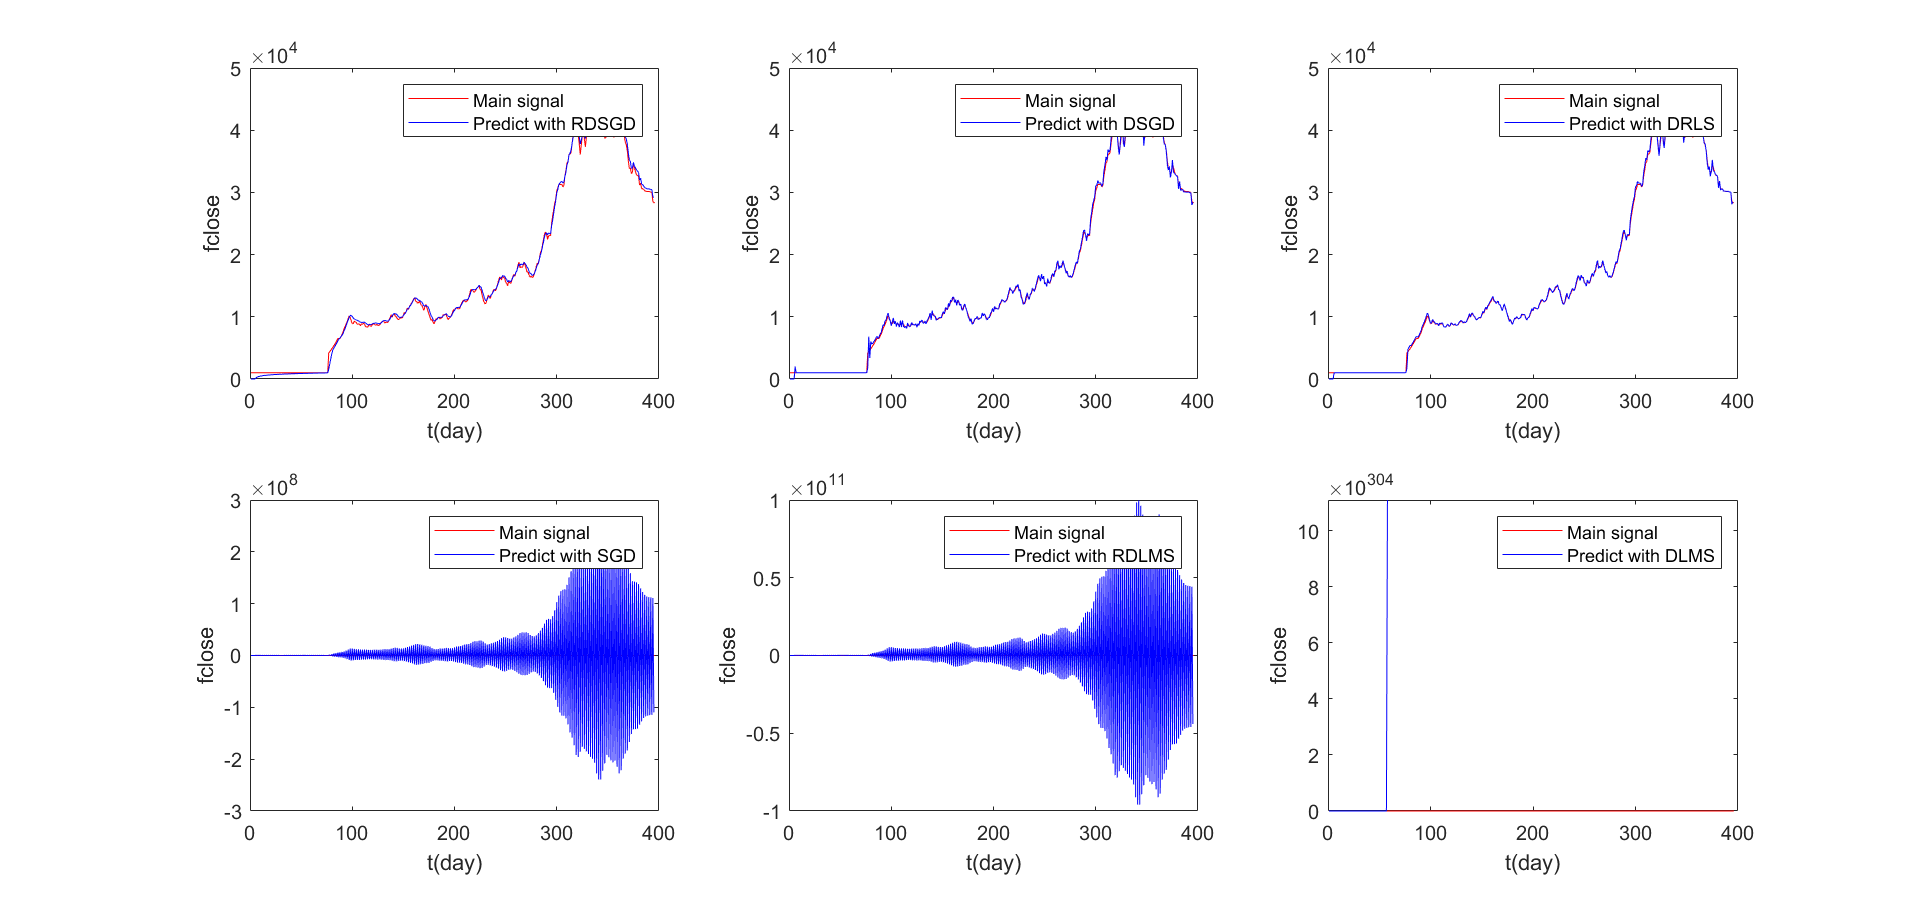
\includegraphics[width=16cm]{ZSharif_Pre.png}
	\caption{مقایسه الگوریتم‌های یادگیری توزیع‌شده رویکرد \lr{FBSP} در پیش‌بینی سیگنال بازار سهام شرکت کشت و صنعت شریف آباد}
	\label{PredictCompare4}
\end{figure*}

\section{خلاصه}
در این فصل، الگوریتم‌های پیشنهادی و رویکرد پیشنهادی روی مسائل شناسایی سیستم و پیش‌بینی داده‌های بورس آزمایش شدند. برای مقایسه با سایر روش‌ها چند معیار ارزیابی و چند روش مقایسه مورد استفاده قرار گرفت. در طی چندین آزمایش، عوامل متعدد و پارامترهای موثر بر کارایی رویکرد پیشنهادی مورد بررسی قرار گرفت. در اولین بررسی انجام شده، تاثیر الگوریتم یادگیری توزیع‌شده مبتنی بر \lr{SGD} بر سرعت همگرایی و دقت یادگیری در مساله بهینه‌سازی شناسایی سیستم نشان داده شد. در واقع الگوریتم پیشنهادی تاثیر چشم‌گیری در کاهش خطا در حالت پایدار داشت. در بررسی دیگر، تاثیر توابع زیان بر مقاومت الگوریتم یادگیری پیشنهادی در برابر انواع نویزهای گاوسی و غیرگاوسی و در انواع محیط‌های ایستا و غیرایستا مورد بررسی قرار گرفت و نشان داده شد که الگوریتم یادگیری پیشنهادی با تابع زیان شبه‌هابر (\lr{RDSGD}) مقاومت بهتری ارائه می‌دهد و نسبت به سایر الگوریتم‌های یادگیری با میانگین خطا کمتری در حالت پایدار همگرا می‌شود. 

رویکرد پیشنهادی \lr{FBSP} با استفاده از الگوریتم‌ یادگیری \lr{RDSGD} و منطقه‌بندی گره‌های شبکه توزیع‌شده، اهدافی چون مدیریت محیط‌های اجرایی ناهمگن، کاهش هزینه ارتباطات، کاهش زمان انتظار گره‌ها در طی فرآیند یادگیری و جلوگیری از مساله کندکننده‌ها با حفظ سرعت و دقت همگرایی را دنبال می‌کند. رویکرد پیشنهادی به دلیل منطقه‌بندی شبکه توانایی بالایی در کاهش هزینه ارتباطات و کاهش زمان انتظار گره‌ها برای شبکه‌های غیرخلوت دارد. در اولین آزمایش تاثیر مقدار پارامتر $qIter$ بر همگرایی، میانگین زمان انتظار و میانگین تعداد ارتباطات گره‌ها در محیط غیرایستا و در حضور نویزهای گاوسی، گاوسی آمیخته و آلفا پایدار مورد ارزیابی قرار گرفت و نشان داده شد که با افزایش مقدار پارامتر $qIter$ رویکرد پیشنهادی به میانگین خطا بالاتری همگرا شده اما در مقابل تعداد ارتباطات و زمان انتظار گره‌ها کاهش می‌یابد. به عبارتی میانگین خطا همگرایی رابطه معکوس با میانگین زمان انتظار گره‌ها دارد. رویکرد پیشنهادی به ازای پارامتر کنترلی $qIter=50$ در یک محیط غیرایستا قادر است باعث کاهش $36.73$ درصدی تعداد ارتباطات و کاهش $36.9$ درصدی زمان انتظار گره‌ها شود. این در حالی است که رویکرد پیشنهادی سبب افزایش تنها $13.38$ درصد در میانگین خطا همگرایی در حالت پایدار  شده است. در آزمایش دوم، رویکرد پیشنهادی از جنبه میانگین زمان انتظار و میانگین خطا همگرایی با سایر رویکردهای مشابه مورد مقایسه قرار گرفت و رویکرد پیشنهادی با پارامتر کنترلی $qIter=50$ به سایر رویکردها غلبه کرد. در آزمایشی دیگر، مقاومت رویکرد پیشنهادی در برابر محیط‌های اجرایی ناهمگن مختلف مورد بررسی قرار گرفت و نشان داده شده که رویکرد \lr{FBSP} از مقاومت بالایی در محیط‌های ناهمگن نسبت به رویکرد مشابه خویش \lr{PSP} دارد. در آزمایش آخر نشان داده شده که رویکرد پیشنهادی با الگوریتم یادگیری توزیع‌شده انتشاری \lr{RDSGD} در مساله پیش‌بینی داده‌های بورس نیز موفق است.

